\documentclass[,man,floatsintext]{apa6}
\usepackage{lmodern}
\usepackage{amssymb,amsmath}
\usepackage{ifxetex,ifluatex}
\usepackage{fixltx2e} % provides \textsubscript
\ifnum 0\ifxetex 1\fi\ifluatex 1\fi=0 % if pdftex
  \usepackage[T1]{fontenc}
  \usepackage[utf8]{inputenc}
\else % if luatex or xelatex
  \ifxetex
    \usepackage{mathspec}
  \else
    \usepackage{fontspec}
  \fi
  \defaultfontfeatures{Ligatures=TeX,Scale=MatchLowercase}
\fi
% use upquote if available, for straight quotes in verbatim environments
\IfFileExists{upquote.sty}{\usepackage{upquote}}{}
% use microtype if available
\IfFileExists{microtype.sty}{%
\usepackage{microtype}
\UseMicrotypeSet[protrusion]{basicmath} % disable protrusion for tt fonts
}{}
\usepackage{hyperref}
\hypersetup{unicode=true,
            pdftitle={Learning Linguistic Disjunction},
            pdfauthor={Masoud Jasbi, Akshay Jaggi, \& Michael C. Frank},
            pdfkeywords={keywords},
            pdfborder={0 0 0},
            breaklinks=true}
\urlstyle{same}  % don't use monospace font for urls
\usepackage{longtable,booktabs}
\usepackage{graphicx,grffile}
\makeatletter
\def\maxwidth{\ifdim\Gin@nat@width>\linewidth\linewidth\else\Gin@nat@width\fi}
\def\maxheight{\ifdim\Gin@nat@height>\textheight\textheight\else\Gin@nat@height\fi}
\makeatother
% Scale images if necessary, so that they will not overflow the page
% margins by default, and it is still possible to overwrite the defaults
% using explicit options in \includegraphics[width, height, ...]{}
\setkeys{Gin}{width=\maxwidth,height=\maxheight,keepaspectratio}
\IfFileExists{parskip.sty}{%
\usepackage{parskip}
}{% else
\setlength{\parindent}{0pt}
\setlength{\parskip}{6pt plus 2pt minus 1pt}
}
\setlength{\emergencystretch}{3em}  % prevent overfull lines
\providecommand{\tightlist}{%
  \setlength{\itemsep}{0pt}\setlength{\parskip}{0pt}}
\setcounter{secnumdepth}{0}
% Redefines (sub)paragraphs to behave more like sections
\ifx\paragraph\undefined\else
\let\oldparagraph\paragraph
\renewcommand{\paragraph}[1]{\oldparagraph{#1}\mbox{}}
\fi
\ifx\subparagraph\undefined\else
\let\oldsubparagraph\subparagraph
\renewcommand{\subparagraph}[1]{\oldsubparagraph{#1}\mbox{}}
\fi

%%% Use protect on footnotes to avoid problems with footnotes in titles
\let\rmarkdownfootnote\footnote%
\def\footnote{\protect\rmarkdownfootnote}


  \title{Learning Linguistic Disjunction}
    \author{Masoud Jasbi\textsuperscript{1}, Akshay Jaggi\textsuperscript{2}, \& Michael C. Frank\textsuperscript{2}}
    \date{}
  
\shorttitle{Learning Linguistic Disjunction}
\affiliation{
\vspace{0.5cm}
\textsuperscript{1} Harvard University\\\textsuperscript{2} Stanford University}
\keywords{keywords\newline\indent Word count: X}
\usepackage{csquotes}
\usepackage{upgreek}
\captionsetup{font=singlespacing,justification=justified}

\usepackage{longtable}
\usepackage{lscape}
\usepackage{multirow}
\usepackage{tabularx}
\usepackage[flushleft]{threeparttable}
\usepackage{threeparttablex}

\newenvironment{lltable}{\begin{landscape}\begin{center}\begin{ThreePartTable}}{\end{ThreePartTable}\end{center}\end{landscape}}

\makeatletter
\newcommand\LastLTentrywidth{1em}
\newlength\longtablewidth
\setlength{\longtablewidth}{1in}
\newcommand{\getlongtablewidth}{\begingroup \ifcsname LT@\roman{LT@tables}\endcsname \global\longtablewidth=0pt \renewcommand{\LT@entry}[2]{\global\advance\longtablewidth by ##2\relax\gdef\LastLTentrywidth{##2}}\@nameuse{LT@\roman{LT@tables}} \fi \endgroup}


\usepackage{lineno}

\linenumbers

\authornote{Add complete departmental affiliations for each author here. Each new line herein must be indented, like this line.

Enter author note here.

Correspondence concerning this article should be addressed to Masoud Jasbi, Postal address. E-mail: \href{mailto:masoud_jasbi@fas.harvard.edu}{\nolinkurl{masoud\_jasbi@fas.harvard.edu}}}

\abstract{
Research on word learning has discovered constraints, cues, and mechanisms that can help a language learner create successful word-meaning mappings. So far, the literature has mainly focused on the acqusition of content words such as nominals and verbs, leaving functional elements largely understudied. The current study fills this gap by investigating the constraints, cues, and mechanisms that can aid the acqusition of disjunction. Based on naturalistic recordings of parent-child interactions, we argue that children may learn to interpret a disjunction by partition their form-meaning mappings based on salient cues that accompany it in child-directed speech. We first show that children start producing \emph{or} between 18-30 months and by 42 months their productions plateau at a constant rate. We also find that the most likely interpretation of \emph{or} in child-directed speech is exclusive disjunction. However, exclusive interpretations correlated with a rise-fall intonation, and logically inconsistent propositions. In the absence of these two cues, \emph{or} was commonly not exclusive. Our computational modeling shows that a hypothetical learner can successfully interpret an English disjunction by mapping forms to meanings after partitioning the input using the set of salient cues (cue-based) in the context of the utterance (context-depenent). We discuss the implications of our work for current theories of word learning.


}

\begin{document}
\maketitle

\hypertarget{introduction}{%
\section{Introduction}\label{introduction}}

Word learning is the process of detecting a word form, hypothesizing candidate meanings, and mapping the word to its correct meaning (Clark, 1993). As Quine (1960) explained, this process is theoretically complex. Consider a child seeing her father pointing to a fish tank and saying: \enquote{\emph{mahi}}! As you probably noticed, \emph{mahi} can mean many things in this context. From \enquote{water}, \enquote{fish}, \enquote{tail}, \enquote{smelly}, and \enquote{look} to \enquote{no touching}, \enquote{few bubbles}, and even more complex concepts like \enquote{fish-during-the-day} or \enquote{fish-water-bubble}. Quine argued that the meanings of linguistic utterances are always underdetermined by the behavioral data available to the learner. This problem is known as \enquote{the mapping problem}, \enquote{the gavagai problem}, or \enquote{indeterminacy of reference}.

There are three general ways of tackling this problem. First, word learning may place a priori \textbf{constraints} or biases on the hypothesis space (Markman, 1990; Markman \& Hutchinson, 1984; Markman \& Wachtel, 1988). For example, children may initially assume that words refer to the whole object rather than its parts. Such a constraint would avoid mapping \emph{mahi} to concepts like \enquote{tail} or \enquote{eye}. In addition, children may assume that new words extend to taxonimically related objects and not thematically related ones, therefore avoiding mapping to a concept like \enquote{fish-water-bubble}. Finally, if the child already knows the word for \enquote{water}, they may assume that \emph{mahi} cannot be the word for the same concept.

Second, linguistic or sociopragmatic \textbf{cues} can add bias for or against some hypotheses. Suppose instead of just saying \enquote{\emph{mahi}}, the father said \enquote{\emph{mahi ro bebin!}}. If the child knows \enquote{\emph{\_\_\_ + ro + bebin}} as a noun + article + verb combination, then she can analyze \emph{mahi} as a noun and limit its candidate meanings to nominal concepts. If she also knows that \enquote{\emph{bebin}} means \enquote{look at}, she can further limit the candidate meanings to things she can actually look at in the scene. Therefore, prior syntactic or semantic knowledge can cue the meaning of an unknown word (Brown, 1957; Gleitman, 1990). Prior knowledge of communicative acts or human social interaction can also inform word learning. For example, the father's pointing to a fish or looking at it while saying \emph{mahi} can also inform the child of what needs to be attended to for understanding the utterance (Baldwin, 1993; Clark, 2009; Tomasello, 2003).

Third, while each learning instance of a word in isolation may be compatible with innumerable candidate meanings, taken together and aggregating \textbf{across situations}, a learner may be able to reduce the indeterminacy substantially (Siskind, 1996; Smith, Smith, \& Blythe, 2011; Yu \& Smith, 2007). For example, the father may later point to the picture of a fish in a story book and say \enquote{\emph{mahi}!} This time there is no \enquote{tank} or \enquote{bubbles}, and the reading may be happening during the night. Therefore, the new observation makes hypotheses like \enquote{tank}, \enquote{few bubbles}, or \enquote{fish-during-the-day} less plausible. If children track which hypotheses fair best across several naming instances, they have a better chance of narrowing down the hypothesis space to the correct meaning.

Constraints, cues, and cross-situational learning can also operate in conjunction in language acquisition (Hollich et al., 2000). Furthermore, the role and prominence of each factor may vary for different classes of words. So far, nominals have received most of the attention in research on cues and constraints that aid word learning. Function words, on the other hand, have remained largely understudied. In this study, we focus on the role of constraints, cues, and cross-situational word learning on the acquistiion of the disjunction word \emph{or}. In the next two parts of this section, we first summarize previous work on the acquisition of disjunction, and second, summarize our account based on the data presented in the current study.

\hypertarget{previous-studies}{%
\subsection{Previous Studies}\label{previous-studies}}

To our knowledge, only one study has looked at spontaneous productions of \emph{and} and \emph{or} in parents' and children's speech. Morris (2008) investigated children between the ages of 2;0 and 5;0, using 240 transcriptions of audiotaped exchanges obtained from the CHILDES database. Each connective was analyzed with respect to its frequency, sentence type, and meaning (or use). The study found that overall, \emph{and} was approximately 12.8 times more likely to be produced than \emph{or}. The connective \emph{and} appeared predominantly in statements (more than 90\% of the time) while \emph{or} was most common in questions (more than 85\% of the time). Children started producing \emph{and} at 2 years and \emph{or} at 2.5 years of age.

Regarding the meaning of the connectives, Morris (2008) adopted a usage-based (item-based) approach (Levy \& Nelson, 1994; Tomasello, 2003) and predicted that children start producing connectives with a single \enquote{core meaning} (also referred to as \enquote{use} or \enquote{communicative function}). He predicted that the core meaning mirrors the most frequent meaning of the connective in child-directed speech. Children acquire the less frequent meanings of the connectives as they grow older. He found that children started producing \emph{and} as conjunction at 2, and \emph{or} as exclusive disjunction at 2.5 years of age. In line with the predictions of the usage-based account, he found that these two meanings are the most frequent meanings in parents' speech. For disjunction, 75-80\% of the \emph{or}-examples children heard recevied an exclusive interpretation. Finally, as children grew older, they started using connectives to convey additional meanings such as inclusive disjunction for \emph{or} and temporal conjunction for \emph{and}. Overall in adult speech, the inclusive use of \emph{or} was extremely rare, and children barely produced it even at age 5. Morris (2008) argued that the development of connectives conforms to the predictions of a usage-based account and that in the first five years of children's development, the (core) meaning of disjunction is exclusive.

However, a series of experimental studies have found that preschool children are more likely to interpret \emph{or} as inclusive in a variety of linguistic contexts such as negative sentences (Crain, Gualmini, \& Meroni, 2000), conditional sentences (Gualmini, Crain, \& Meroni, 2000), restriction and nuclear scope of the universal quantifier \emph{every} (Chierchia, Crain, Guasti, Gualmini, \& Meroni, 2001; Chierchia et al., 2004), nuclear scope of the negative quantifier \emph{none} (Gualmini \& Crain, 2002), restriction and nuclear scope of \emph{not every} (Notley et al., 2012a), and prepositional phrases headed by \emph{before} (Notley et al., 2012b). These studies almost unanimously claim that at least in declarative sentences, the inclusive interpretation of \emph{or} emerges earlier than the exclusive interpretation.

The findings of these studies and Morris (2008) give rise to a paradox: how can children learn to interpret linguistic disjunction as inclusive, if they rarely hear it as inclusive? One way to addresses this paradox is logical nativism (Crain, 2012; Crain \& Khlentzos, 2008, 2010). It proposes that the language faculty constrains the connective meanings entertained by the learner to those used in classical logic: negation, conjunction, and inclusive disjunction. Crain (2012) considered it unlikely that children learn the meaning of \emph{or} from the examples they hear in adult usage. Instead, he argued that children rely on an innate knowledge that the meaning of disjunction words in natural languages must be inclusive. In other words, upon hearing a connective word, children consider inclusive disjunction as a viable candidate for its meaning but not exclusive disjunction. In this account, the exclusive interpretation emerges as part of children's pragmatic development after they have mastered the inclusive semantics of disjunction.

While logical nativism addresses the paradox of learning disjunction, it does not provide an explanation for cases where children interpret disjunction as exclusive. Morris (2008) reported that in his study, the vast majority of children used \emph{or} in its exclusive sense. This is not expected if preschool children consider disjunction to be inclusive. Second, other experimental studies, especially those testing disjunction in commands, find that preschool children interpret it as exclusive (Braine \& Rumain, 1981; Johansson \& Sjolin, 1975). For example, in response to a command such as \enquote{give me the doll or the dog}, children as young as three- and four-years-old give one of the objects and not both. In its current version, the nativist account does not explain such cases.

Figure \ref{fig:theories} summarizes the usage-based and nativist approaches to the acquisition of disjunction. The major difference between them is their assumptions on the learners' semantic hypothesis space for \emph{or}. The usage-based account considers a wide array of meanings to be available for mapping, including different flavors of conjunction such as \enquote{temporal conjunction} (e.g.~Bob pressed the key and (then) the door opened) and \enquote{explanatory conjunction}. The nativist account places more constraints ont the hypothesis space and limits it to binary logical connectives of standard propositional logic: inclusive disjunction, conjunction, and material implication. Both accounts agree that the input favors the exclusive interpretation of disjunction. The usage-based account concludes that children's early mappings mirror this input. The nativist account suggests that innate biases towards the inclusive meaning and against the exclusive interpretation result in an inclusive semantics for \emph{or} in children's early mappings.

\begin{figure}[tb]

{\centering 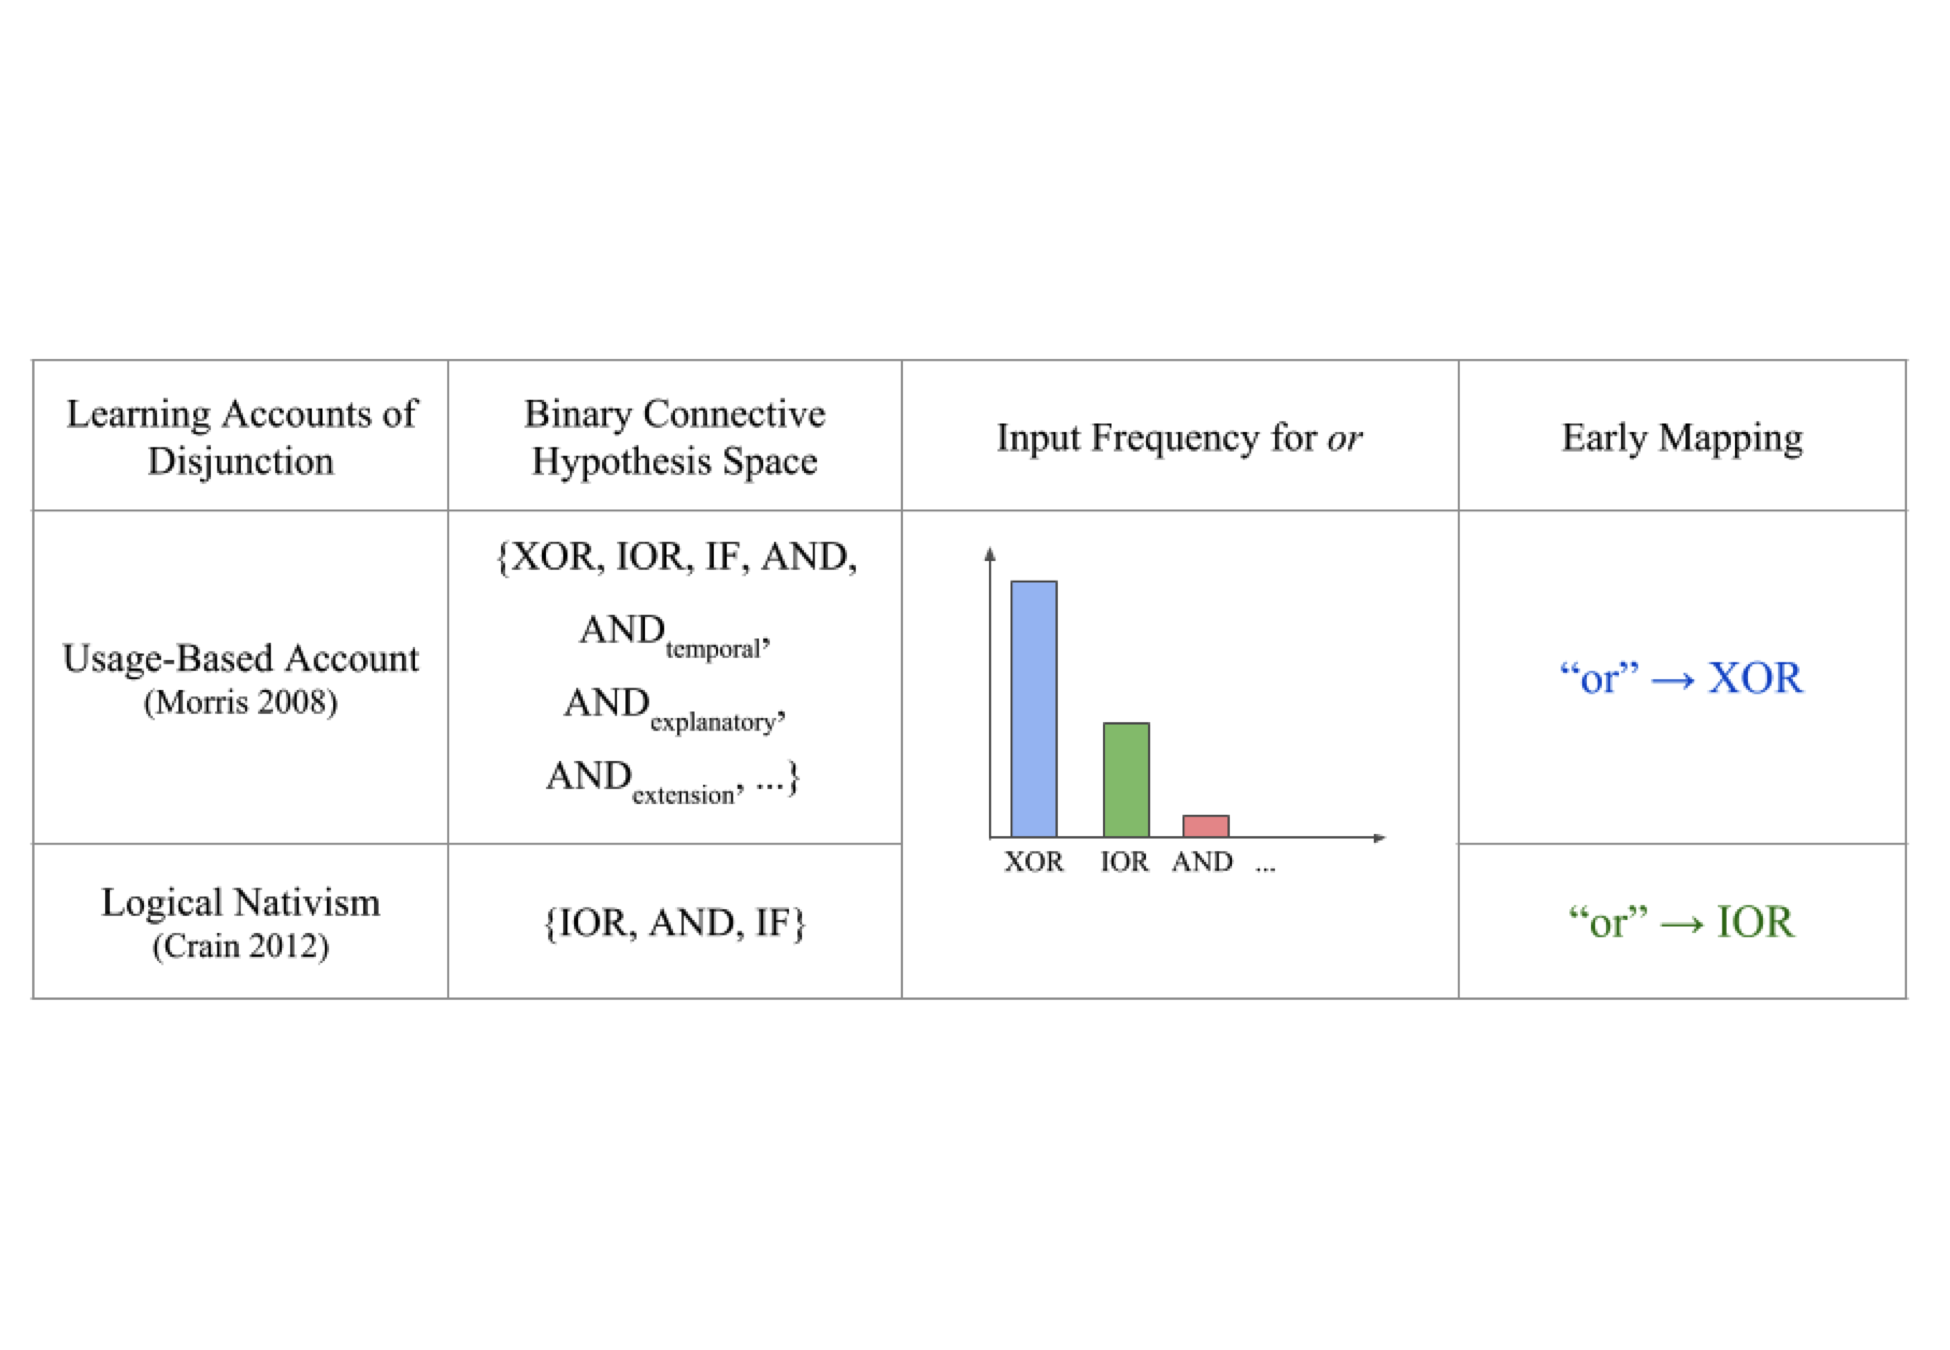
\includegraphics{figs/theories-1} 

}

\caption{Summary of the usage-based and nativist approaches to the acquisition of disjunction.}\label{fig:theories}
\end{figure}

\hypertarget{current-study}{%
\subsection{Current Study}\label{current-study}}

In this study, we provide an alternative solution to the paradox of learning disjunction. The main claim of this paper is that child-directed speech contains salient cues that accompany a linguistic disjunction and can help a learner successfully interpret it -- for example as exclusive or inclusive. We support this hypothesis using three studies. Study 1 does not directly support our main claim but provides the necessary basic information. It investigates the distribution of \emph{and} and \emph{or} in parent-child interactions to address the following basic questions: how often do children hear or produce \emph{or}? and when do they start producing it? Using a large corpus of parent-child interactions, we found that children hear 1-2 examples of \emph{or} in every thousand words parents produce. They start producing it themselves between 18-30 months, and by 42 months they reach a rate of one \emph{or} per thousand words. Studies 2 and 3 provide support for the two parts of our main claim: presence of cues, and their utility in learning. In study 2, we ask: what interpretations can \emph{or} have in child-directed speech? We annotated examples of \emph{or} and found that its most likely interpretation is exclusive disjunction, as Morris (2008) had concluded. However, we also found that exclusive interpretations correlated strongly with two cues: rise-fall prosody, and logically inconsistent propositions connected by \emph{or}. In the absence of these cues, \emph{or} was most likely non-exclusive. In our third study, we asked if it is possible to learn the interpreations of \emph{or} from these cues. Using the annotation data of study 2 and a supervised learning task, we showed that a decision-tree classifer can use prosody and consistency of propositions to predict its interpretation with high accuracy.

Based on the results of our studies, we propose a new account for children's acquisition of disjunction. Figure \ref{fig:cueBasedAccount} shows the summary of this account which we call \enquote{cue-based context-dependent mapping} of disjunction. It is inspired by the usage-based and nativist accounts of disjunction and shares many of their insights. Similar to the nativist account, we assume that the semantic hypothesis space includes binary logical relations. However, we do not limit the hypothesis space further and do not bias the learning towards the inclusive meaning. We will show that the linguistic input can achieve this. Similar to usage based proposals, our account relies on the structure of the input to distinguish between exclusive and inclusive uses of disjunction. We also map more complex constructions to meanings rather than the word \emph{or} directly. The learner can later extract commonalities across mappings to complex forms and extract a core semantics for a particular word like \emph{or}. The major point of departure from previous accounts is the mechanism of learning. While in pervious accounts the most frequent meaning in the input was mapped to the connective word directly, in our account the input is partitioned or broken down by a set of salient cues that designate the context of use. Mapping is done based on the cues that accompany the connective word.

\begin{figure}[tb]

{\centering 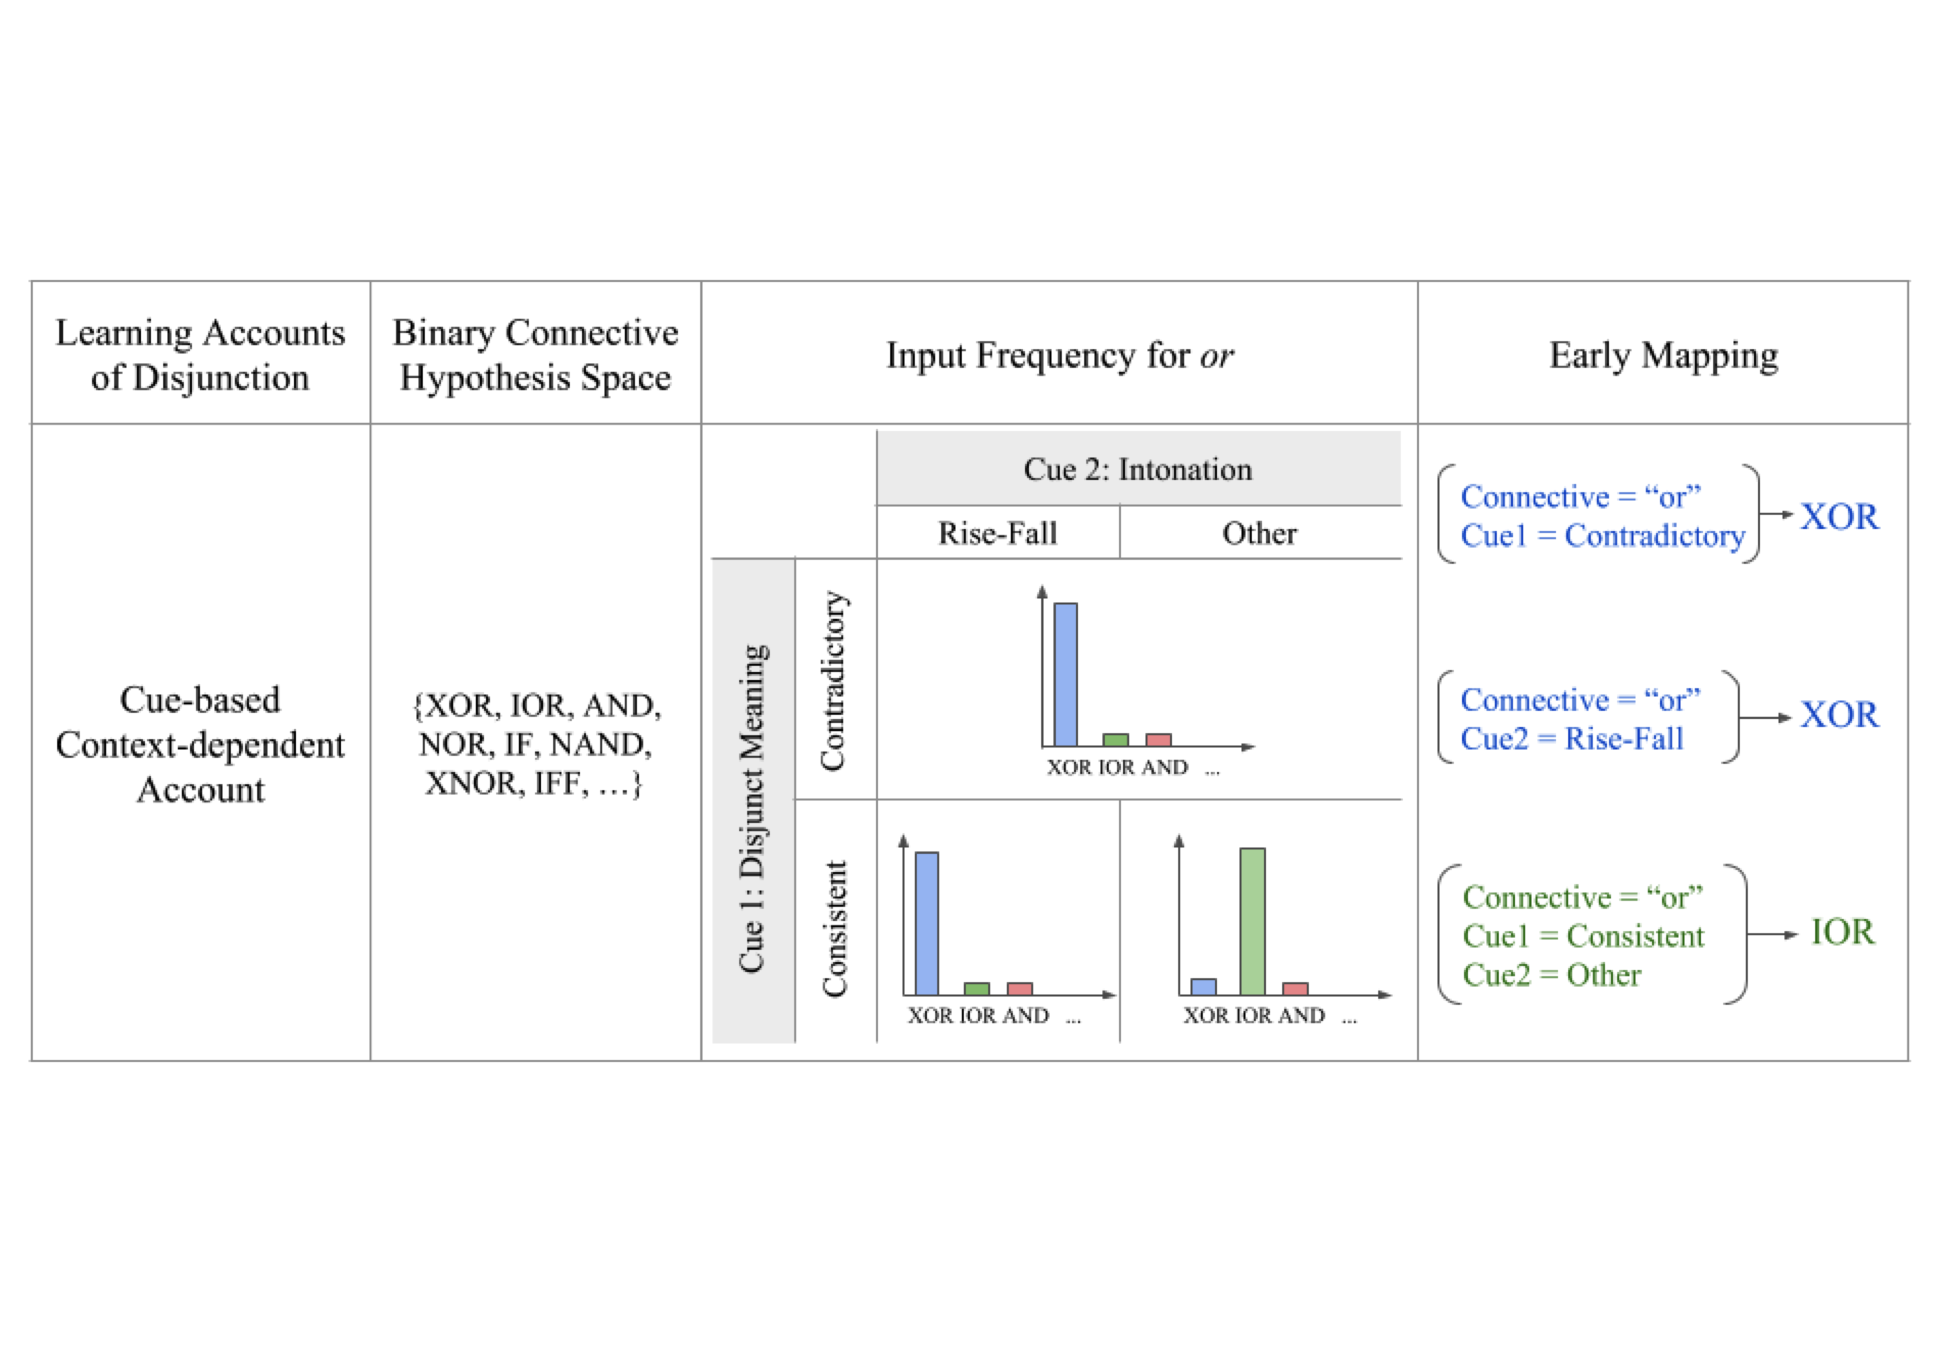
\includegraphics{figs/cueBasedAccount-1} 

}

\caption{Summary of the usage-based and nativist approaches to the acquisition of disjunction.}\label{fig:cueBasedAccount}
\end{figure}

\hypertarget{study-1-production-of-or-in-parent-child-interactions}{%
\section{\texorpdfstring{Study 1: Production of \enquote{or} in parent-child interactions}{Study 1: Production of ``or'' in parent-child interactions}}\label{study-1-production-of-or-in-parent-child-interactions}}

In our first study, we looked at the frequencies of \emph{and} and \emph{or} in a corpus of parent-child interactions (CHILDES) with 14,159,609 words. This is a considerably larger corpus than previously used.

\hypertarget{methods}{%
\subsection{Methods}\label{methods}}

For samples of parents' and children's speech, we used the online database \href{childes-db.stanford.edu}{childes-db} and its associated R programming package \texttt{childesr} (Sanchez et al., 2018). Childes-db is an online interface to the child language components of \href{https://talkbank.org/}{TalkBank}, namely \href{https://childes.talkbank.org/}{CHILDES} (MacWhinney, 2000) and \href{https://phonbank.talkbank.org/}{PhonBank}. Two collections of corpora were selected: English-North America and English-UK. All word tokens were tagged for the following information: 1. The speaker role (mother, father, child), 2. the age of the child when the word was produced, 3. the type of the utterance the word appeared in (declarative, question, imperative, other), and 4. whether the word was \emph{and}, \emph{or}, or neither.

\hypertarget{exclusion-criteria}{%
\subsubsection{Exclusion Criteria}\label{exclusion-criteria}}

First, tokens were coded as unintelligible were excluded (N = 290,119). Second, tokens that had missing information on children's age were excluded (N = 1,042,478). Third, tokens outside the age range of 1 to 6 years were excluded (N = 686,870). We were interested in the 1 to 6 years old age range and there was not much data outside this age range. The collection contained the speech of 504 children and their parents after the exclusions.

\hypertarget{procedure}{%
\subsubsection{Procedure}\label{procedure}}

Each token was marked for the utterance type that the token appeared in. This study grouped utterance types into four main categories: \enquote{declarative}, \enquote{question}, \enquote{imperative}, and \enquote{other}. Utterance type categorization followed the convention used in the \href{https://talkbank.org/manuals/CHAT.html\#_Toc486414422}{TalkBank manual}. The utterance types are similar to sentence types (declarative, interrogative, imperative) with one exception: the category \enquote{question} consists of interrogatives as well as rising declaratives (i.e.~declaratives with rising question intonation). In the transcripts, declaratives are marked with a period, questions with a question mark, and imperatives with an exclamation mark. It is important to note that the manual also provides \href{https://talkbank.org/manuals/CHAT.html\#_Toc486414431}{terminators for special-type utterances}. Among the special type utterances, this study included the following in the category \enquote{questions}: trailing off of a question, question with exclamation, interruption of a question, and self-interrupted question. The category imperatives also included \enquote{emphatic imperatives}. The rest of the special type utterances such as \enquote{interruptions} and \enquote{trailing off} were included in the category \enquote{other}.

\hypertarget{study1results}{%
\subsection{Results}\label{study1results}}

Overall, \emph{and} was about 10 times more likely to occur in parents' speech than \emph{or}. More specifically, \emph{and} occurred 15 times and \emph{or} only 1.5 times per 1000 words. Children produced \emph{and} at the same rate as their parents but produced \emph{or} at a considerably lower rate, only 0.5 per thousand (Figure \ref{fig:freqPlots}, Left). The developmental trend showed that between 12 to 72 months, production of \emph{and} in parents' speech varied between 10 to 20 per thousand words (Figure \ref{fig:freqPlots}, Right). Children started producing \emph{and} between 12 and 18 months, and showed a sharp increase in their production until they reached the parent level between 30 to 36 months of age. Their productions stayed close to the parents' production level between 36 and 72 months, possibly surpassing them at 60 months -- although due to the small amount of data after 60 months we should be cautious with our interpretation of the trend there. The production of \emph{or} for parents was 1 to 2 per thousand words. Children started producing \emph{or} between 18 to 30 months, steadily increasing their productions until they got close to 1 \emph{or} per thousand words at 48 months (4 years). Their productions plateaued and stayed at this rate until 72 months (6 years).

\begin{figure}[tb]

{\centering 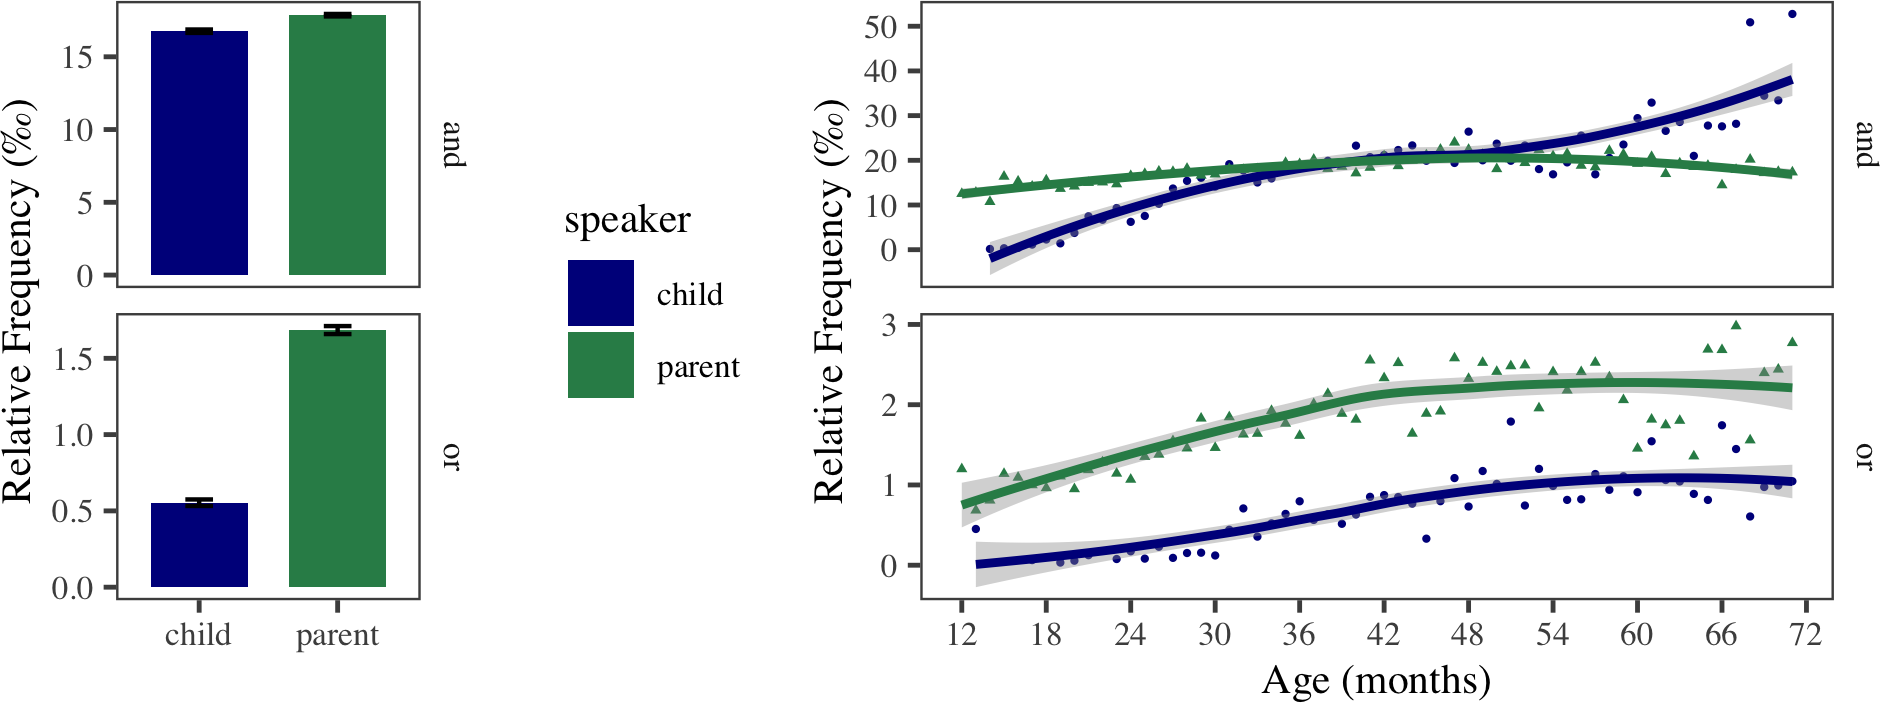
\includegraphics{figs/freqPlots-1} 

}

\caption{Left: The relative frequency of \textit{and/or} (per mille) in the speech of parents and children. 95\% binomial proportion confidence intervals calculated using Agresti-Coull's approximate method. Right: The monthly relative frequency of \textit{and/or} in parents and children's speech between 12 and 72 months (1-6 years).}\label{fig:freqPlots}
\end{figure}

Children's productions of \emph{or} was different from their production of \emph{and} and parents' production of \emph{or}. Children started producing \emph{or} around 6 months later than they started with \emph{and}. Second, while children's \emph{and} productions showed a steep rise over a year and reached the parent level around 30 months, their \emph{or} productions rose slowly and did not reach the parent level even at 6 years of age. What factors cause these differences? We consider three possibilities here: frequency, conceptual complexity, and usage.

First, \emph{and} is a far more frequent connective than \emph{or}. Goodman, Dale, and Li (2008) argue that within the same syntactic category, words with higher frequency in child-directed speech are acquired earlier. The conjunction word \emph{and} is at least 10 times more likely to occur than \emph{or} so earlier acquisition of \emph{and} is consistent with the effect of frequency on age of acquisition. Second, research on concept attainment has suggested that the concept of conjunction is easier to conjure and possibly acquire than the concept of disjunction. In experiments that participants are asked to detect the pattern of classification in some cards, they can detect a conjunctive classification faster than a disjunctive one (Neisser \& Weene, 1962). Therefore, it is possible that children discover the concept that corresponds to the meaning of \emph{and} faster and start to produce it earlier, but they need more time to attain the concept corresponding to the meaning of \emph{or}.

A third possibility is that the developmental difference between \emph{and} and \emph{or} is at least partly due to their different usages. Parent-child interactions are not symmetrical and what parents would like to communicate to children is different from what children would like to communicate to parents. This asymmetry can result in different distribution of speech acts between parents and children and consequently functional elements that constitute them. Here we present evidence that suggests \emph{or} is affected in this way.

\begin{figure}[tb]

{\centering 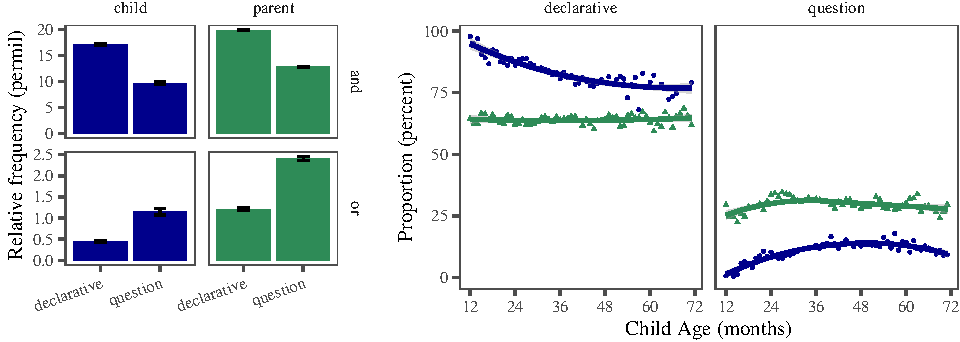
\includegraphics{figs/speechActPlots-1} 

}

\caption{Left: Relative frequency of \textit{and/or} (per mille) in declaratives, imperatives, and interrogatives for parents and children. Right: Percentage of declaratives to questions in parent-child interactions by age.}\label{fig:speechActPlots}
\end{figure}

First, we found that \emph{or} was more likely to occur in questions than in declaratives (Figure \ref{fig:speechActPlots}, Left). This is in contrast to \emph{and} which was more likely to occur in declaratives. Second, parents asked more questions from children than children did from parents, and children produced more declaratives than parents (Figure \ref{fig:speechActPlots}, Right). In fact, questions had their own developmental trajectory, emerging in the second year of children's lives and reaching a relatively constant rate of about 15\% of children's utterances in their fourth year. However, parents produce a constant rate of questions which is about 25\% of their utterances. Therefore, parent-child interaction provides more opportunities for parents to ask questions and produce \emph{or}, than children.

\begin{figure}[tb]

{\centering 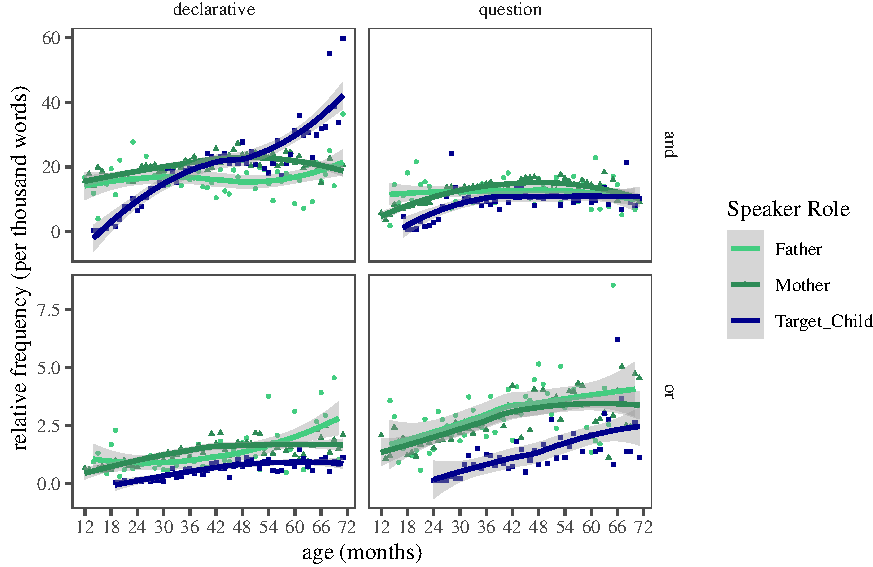
\includegraphics{figs/ageSpeechActPlot-1} 

}

\caption{Relative frequency of \textit{and/or} in declaratives and questions for parents and childern between the child-age of 12 and 72 months (1-6 years).}\label{fig:ageSpeechActPlot}
\end{figure}

Figure \ref{fig:ageSpeechActPlot} shows the developmental trends for the relative frequencies of \emph{and} and \emph{or} in questions and declaratives. Comparing \emph{and} in declaratives and questions, we see that the onset of \emph{and} productions were slightly delayed for questions. But in both declaratives and questions, \emph{and} productions reached the parent level around 30 months (2.5 years). For \emph{or}, we see a similar delay in questions compared to declaratives. Children started producing \emph{or} in declaratives at around 18 months but they started producing \emph{or} in questions at 24 months. Production of \emph{or} increased in both declaratives and questions until it reached a constant rate in declaratives between 48 and 72 months. The relative frequency of \emph{or} in questions continued to rise until 60 months. Comparing Figure \ref{fig:freqPlots} and \ref{fig:ageSpeechActPlot}, children were closer to the adult rate of production in declaratives than questions.

\begin{table}[t]

\caption{\label{tab:study1coeftable}Estimated cofficients for the linear model with children's age, speaker (child vs. parent), utterance type (declarative vs. question), and their interactions as predictors. Relative frequency of disjunction produciton was the dependent variable.}
\centering
\fontsize{9}{11}\selectfont
\begin{tabular}{l|r|r|r|r}
\hline
Coefficients & Estimate & Std. Error & t value & Pr(>|t|)\\
\hline
age & 0.02 & 0.01 & 3.54 & 0.00\\
\hline
question & -0.77 & 0.39 & -1.96 & 0.05\\
\hline
parent & 0.72 & 0.32 & 2.24 & 0.03\\
\hline
age*question & 0.03 & 0.01 & 3.96 & 0.00\\
\hline
age*parent & 0.00 & 0.01 & 0.21 & 0.83\\
\hline
question*parent & 1.40 & 0.48 & 2.91 & 0.00\\
\hline
age*question*parent & -0.01 & 0.01 & -1.30 & 0.20\\
\hline
\end{tabular}
\end{table}

To test these observations more formally, we used a linear regression model with the relative frequency of \emph{or} as the dependent variable and children's age, speaker (child vs.~parent), utterance type (declarative vs.~question), and their interactions as predictors. The intercept was set to children's productions in declaratives. Table \ref{tab:study1coeftable} presents the coefficient estimates of the model. Overall, the model suggests that parents and children produced more \emph{or} as children grew older and parents produced more instances of \emph{or} than children. However, the increase in production of \emph{or} was more steep in questions. The largest significant effect was the interaction of speaker and utterance type. Parents produced disjunctions more frequently in quesions than in declaratives. These results are consistent with the hypothesis that frequency and distribution of \emph{or} is partly affected by the development of questions in parent-child interactions.

\hypertarget{study1discussion}{%
\subsection{Conclusion}\label{study1discussion}}

In a large-scale quantitative analysis of parents and children's productions of \emph{and} and \emph{or}, we found that children started producing \emph{and} in the second year of their lives, and quickly reached their parents' rate of production by two and a half. Their production of disjunction was delayed by six months on average: they started producing \emph{or} between 1.5 and 2.5 years of age, and around 3.5 years, they reached a relatively constant rate of production below that of their parents. We considered three possible causes for disjunction's delay and lower rate of production: the higher frequency of \emph{and}, the conceptual and mapping complexity of \emph{or}, and the asymmetry in speech acts produced by parents and children. We provided evidence for the last cause. We showed that parents produced more questions than children, and that \emph{or} was more likelly to occur in questions. Therefore, parents' speech contained more \emph{or} partly due to the fact that parents asked more questions.

\hypertarget{study-2-interpretations-of-disjunction-in-child-directed-speech}{%
\section{Study 2: Interpretations of disjunction in child-directed speech}\label{study-2-interpretations-of-disjunction-in-child-directed-speech}}

In this study we selected a subset of connective examples in child-directed speech from study 1 to closely examine the interpretations they recieve. Research in formal semantics has shown that the interpretation of disjunction depends on several factors including prosody (Pruitt \& Roelofsen, 2013), logical consistency of the propositions being connected (Geurts, 2006), pragmatic and scalar reasoning (Grice, 1989). Our main claim here is that in child-directed speech, exclusive interpretations of \emph{or} correlate with rise-fall prosody and logically inconsistent propositions. In the absence of these two factors, \emph{or} is most likely \enquote{not exclusive}.

\hypertarget{methods-1}{%
\subsection{Methods}\label{methods-1}}

This study used \href{https://phonbank.talkbank.org/browser/index.php?url=Eng-NA/Providence/}{the Providence corpus} (Demuth, Culbertson, \& Alter, 2006) available via the \href{https://phonbank.talkbank.org}{PhonBank} section of \href{https://talkbank.org/}{the TalkBank.org archive}. The corpus was chosen because of its relatively dense data on child-directed speech as well as the availability of audio and video recordings that would allow annotators access to the context of the utterance. The corpus was collected between 2002 and 2005 in Providence, Rhode Island. Table \ref{tab:providence} in appendix reports the name, age range, and the number of recording sessions for the children in this study. All children were monolingual English speakers and were followed between the ages of 1 and 4 years. Based on Study 2, this is the age range when children develop their early understanding of \emph{and} and \emph{or}. The corpus contains 364 hours of biweekly hour-long interactions between parents and children.

\hypertarget{exclusion-criteria-1}{%
\subsubsection{Exclusion Criteria}\label{exclusion-criteria-1}}

We excluded data from Ethan since he was diagnosed with Asperger's Syndrome at age 5. We also excluded all examples found in conversations over the phone, adult-adult conversations, and utterances heard from TV or radio. We did not count such utterances as child-directed speech. We excluded proper names and fixed forms such as \enquote{Bread and Circus} (name of a local place) or \enquote{trick-or-treat} from the set of examples to be annotated. Such forms could be learned and understood with no actual understanding of the connective meaning. We counted multiple instances of \emph{or} and \emph{and} within the same disjunction/conjunction as one instance. The reasoning was that, in a coordinated structure, the additional occurrences of a connective typically did not alter the annotation categories, and most importantly the interpretation of the coordination. For example, there is almost no difference between \enquote{cat, dog, and elephant} versus \enquote{cat and dog and elephant} in interpretation. In short, we focused on the \enquote{coordinated construction} as a unit rather than on every separate instance of \emph{and} and \emph{or}. Instances of multiple connectives in a coordination were rare in the corpus.

\hypertarget{procedure-1}{%
\subsubsection{Procedure}\label{procedure-1}}

All utterances containing \emph{and} and \emph{or} were extracted using \href{http://alpha.talkbank.org/clan/}{the CLAN software} and automatically tagged for the following: (1) the name of the child; (2) the transcript address; (3) the speaker of the utterance (father, mother, or child); (4) the child's birth date, and (5) the recording date. Since the focus of the study was mainly on disjunction, we annotated instances of \emph{or} in all the child-directed speech from the earliest examples to the latest ones found. Given that the corpus contained more than 10 times the number of \emph{and}'s than \emph{or}'s, we randomly sampled 1000 examples of \emph{and} to match 1000 examples of \emph{or}. Here we report the results on 627 examples of \emph{and} and 608 examples of \emph{or}.

\hypertarget{annotation-categories}{%
\subsubsection{Annotation Categories}\label{annotation-categories}}

Every extracted instance of \emph{and} and \emph{or} was manually annotated for 7 categories: connective interpretation, intonation type, utterance type, syntactic level, conceptual consistency, communicative function, and answer type. We briefly explain how each annotation category was defined. Further details and examples are provided in the appendix section.

\begin{enumerate}
\def\labelenumi{\arabic{enumi}.}
\tightlist
\item
  \emph{Connective Interpretation}
\end{enumerate}

This annotation category was the dependent variable of the study. Annotators listened to coordinations such as \enquote{A or B} and \enquote{A and B}, and decided the intended interpretation of the connective with respect to the truth of A and B. We used the sixteen binary connective meanings shown in Figure \ref{fig:logicalConnectives}. Annotators were asked to consider the two propositions raised by the coordinated construction, ignoring the connective and functional elements such as negation. Consider the following sentences containing \emph{or}: \enquote{Bob plays soccer or tennis} and \enquote{Bob doesn't play soccer or tennis}. Both discuss the same two propositions: A. Bob playing soccer, and B. Bob playing tennis. However, the functional elements combining these two propositions result in different interpretations with respect to the truth of A and B. In \enquote{Bob plays soccer or tennis} which contains a disjunction, the interpretation is that Bob plays one or possibly both sports (IOR). In \enquote{Bob doesn't play soccer or tennis} which contains a negation and a disjunction, the interpretation is that Bob plays neither sport (NOR). For connective interpretations, the annotators first reconstructed the coordinated propositions without the connectives or negation and then decided which propositions were implied to be true/false.

\begin{figure}[tb]

{\centering 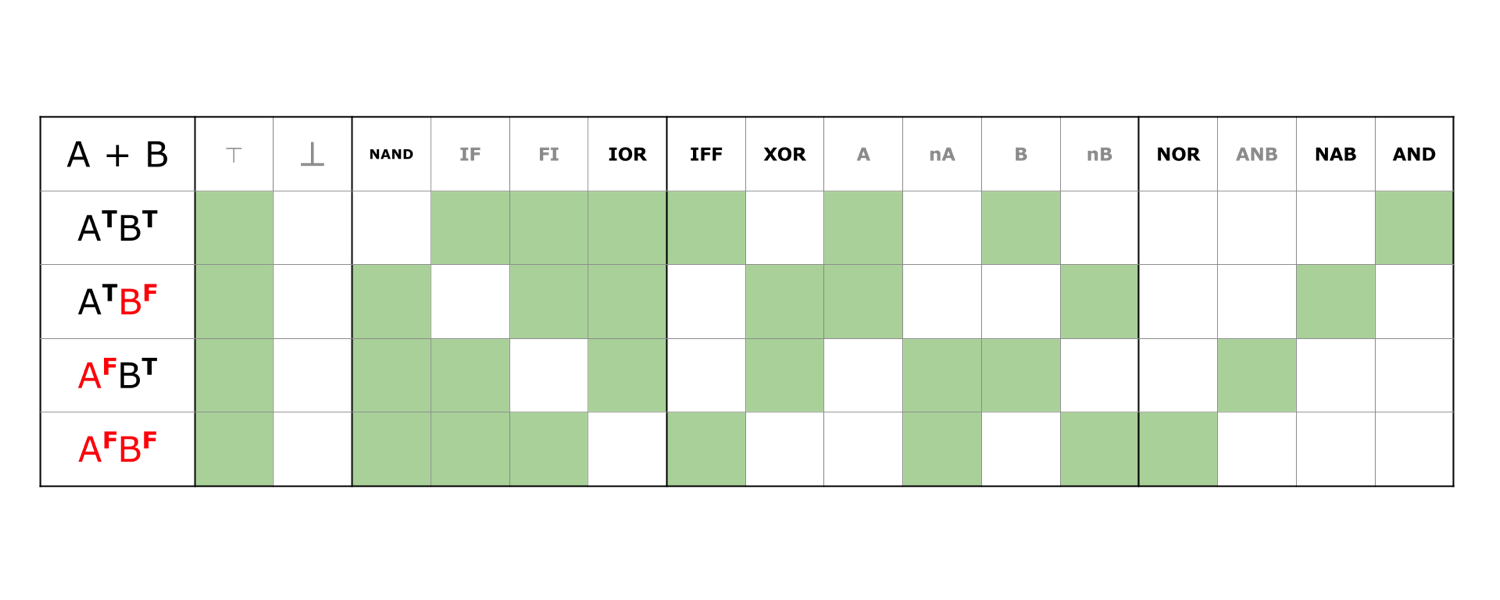
\includegraphics{figs/logicalConnectives-1} 

}

\caption{The truth table for the 16 binary  logical connectives. The rows represent the set of situations where bot A and B, A, B, or, neither propositions are true. The columns represent the 16 possible connectives and their truth conditions. Green cells represent true situations.}\label{fig:logicalConnectives}
\end{figure}

\begin{enumerate}
\def\labelenumi{\arabic{enumi}.}
\setcounter{enumi}{1}
\tightlist
\item
  \emph{Conceptual Consistency}
\end{enumerate}

Propositions stand in complex conceptual relations with each other. For example, have logical, temporal, and causal relation with each other. For conceptual consistency, annotators decided whether the propositions that made up the coordination could be true at the same time or not. If the two propositions could not be true at the same time and resulted in a contradiction, they were marked as inconsistent. Our annotators used the following diagnostic to decide the consistency of the disjuncts: Two disjuncts were marked as inconsistent if replacing the word \emph{or} with \emph{and} produced a contradiction. For example, changing \enquote{the ball is in my room \emph{or} your room} to \enquote{the ball is in my room \emph{and} your room} produces a contradiction because a ball cannot be in two rooms at the same time.

It is important to discuss two issues regarding conceptual consistency. First, our diagnostic for consistency was quite strict. In many cases, propositions are not inconsistent in this sense but they are implausible. For example, drinking both tea and coffee at the same time is not inconsistent, but is unlikely. It is possible that many exclusive interpretations are based on such judgments of implausability. Second, if the coordinands are inconsistent, this does not necessarily mean that the connective interpretation must be exclusive. For example, in a sentence like \enquote{you could stay here or go out}, the alternatives \enquote{staying here} and \enquote{going out} are inconsistent. Yet, the overall interpretation of the connective could be conjunctive: you could stay here AND you could go out. The statement communicates that both possibilities hold. This pattern of interaction between possibility modals like \emph{can} and disjunction words like \emph{or} are often discussed under \enquote{free-choice inferences} in the semantics and pragmatics literature (Kamp, 1973; Von Wright, 1968). Another example is unconditionals such as \enquote{Ready or not, here I come!}. The coordinands are contradictions: one is the negation of the other. However, the overall interpretation of the sentences is that in both cases, the speaker is going to come.

\begin{enumerate}
\def\labelenumi{\arabic{enumi}.}
\setcounter{enumi}{2}
\tightlist
\item
  \emph{Utterance Type}
\end{enumerate}

Annotators decided whether an utterance was an instance of a declarative, an interrogative, or an imperative. Occasionally, we found examples with different utterance types for each coordinand. For example, a mother could say \enquote{put your backpack on and I'll be right back}, where the first cooridnand is an imperative and the second a declarative. Such examples were coded for both utterance types with a dash inbetween: imperative-declarative. Table \ref{tab:utteranceTypes} in the appendix provides the detailed definitions and examples for each utterance type.

\begin{enumerate}
\def\labelenumi{\arabic{enumi}.}
\setcounter{enumi}{3}
\tightlist
\item
  \emph{Intonation Type}
\end{enumerate}

Annotators listened to the utterances and decided whether the intonation contour on the coordination was flat, rise, or rise-fall. Table \ref{tab:intonationTypes} in the appendix shows the definitions and examples for these intonation types. In order to judge the intonation of the sentence accurately, annotators were asked to construct all three intonation contours for the same sentence and see which one is closer to the actual intonation of the utterance. For example, to judge the sentence \enquote{do you want orange juice\(\uparrow\) or apple juice\(\downarrow\)?}, they reconstructed the sentence with the prototypical flat, rising, and rise-fall intonations and checked to see which intonation is closer to the actual one.

\begin{enumerate}
\def\labelenumi{\arabic{enumi}.}
\setcounter{enumi}{4}
\tightlist
\item
  \emph{Syntactic Level}
\end{enumerate}

Annotators marked whether the coordination was at the clausal level or at the sub-clausal level. Clausal level was defined as sentences, clauses, verb phrases, and verbs. Coordination of other categories was coded as sub-clausal. This annotation category was introduced to check the hypothesis that the syntactic category of the coordinands may influence the interpretation of a coordination. For example, a sentence like \enquote{He drank tea or coffee} is less likely to be interpreted as exclusive than \enquote{He drank tea or he drank coffee.} The clausal vs.~sub-clausal distinction was inspired by the fact that in many languages, coordinators that connect sentences and verb phrases are different lexical items than those that connect nominal, adjectival, or prepositional phrases (see Haspelmath, 2007).

\begin{enumerate}
\def\labelenumi{\arabic{enumi}.}
\setcounter{enumi}{5}
\tightlist
\item
  \emph{Communicative Functions}
\end{enumerate}

We constructed a set of categories that captured particular usages or communicative functions of the words \emph{or} and \emph{and}. They include descriptions, directives, preferences, identifications, definitions-examples, clarifications, repairs, and a few others shown in Table \ref{tab:speechActs} in appendix. These communicative functions were created using the first 100 examples and then they were used for the classification of the rest of the examples. Some communicative functions are general and some are specific to coordination. For example, directives are a general class while conditionals (e.g.~Put that out of your mouth, or I'm gonna put it away) are more specific to coordinated constructions. It is also important to note that the list is not unstructured. Some communicative functions are subtypes of others. For example, \enquote{identifications} and \enquote{unconditionals} are subtypes of \enquote{descriptions} while \enquote{conditionals} are a subtype of directives. Furthermore, \enquote{repairs} seem parallel to other categories in that any type of speech can be repaired. We do not fully explore the details of these functions in this study but such details matter for a general theory of acquisition that makes use of the speaker's communicative intentions as early coarse-grained communicative cues for the acquisition of fine-grained meaning such as function words.

\begin{enumerate}
\def\labelenumi{\arabic{enumi}.}
\setcounter{enumi}{6}
\tightlist
\item
  \emph{Answer Type}
\end{enumerate}

Whenever a parent's utterance was a polar question, the annotators coded the utterance for the type of response it received from the children. This annotation category was different from others because it was not used as a cue for learning disjunction. Instead, it was used as an opportunity to assess, albeit in a limited and indirect way, the comprehension of children in the same corpus. Table \ref{tab:answerTypes} in the appendix shows the answer types in this study and their definitions and examples. Utterances that were not polar questions were simply coded as NA for this category. If children responded to polar questions with \enquote{yes} or \enquote{no}, the category was YN and if they repeated with one of the coordinands the category was AB. If children said yes/no and followed it with one of the coordinands, the answer type was determined as YN (yes/no). For example, if a child was asked \enquote{Do you want orange juice or apple juice?} and the child responded with \enquote{yes, apple juice}, our annotators coded the response as YN. The reason is that in almost all cases, if a simple yes/no response is felicitous, then it can also be optionally followed with mentioning a disjunct. However, if yes/no is not a felicitous response, then mentioning one of the alternatives is the only appropriate answer. For example, if someone asks \enquote{Do you want to stay here or go out?} a response such as \enquote{yes, go out} is infelicitous and a better response is simply \enquote{go out}. Therefore, we counted responses with both yes/no and mentioning an alternative as a yes/no response.

\begin{enumerate}
\def\labelenumi{\arabic{enumi}.}
\setcounter{enumi}{7}
\tightlist
\item
  \emph{Negation and Modals}
\end{enumerate}

Finally, a script was used to automatically mark utterances for whether they contain sentential negation (\emph{not}/\emph{n't}) or any modal auxiliary such as \emph{maybe}, \emph{can}, \emph{could}, \emph{should}, \emph{would}, or \emph{need to}. This allowed us to see how the presence or absence of negation or modals could affect the overall interpretation of the utterance.

\hypertarget{inter-annotator-reliability}{%
\subsubsection{Inter-annotator Reliability}\label{inter-annotator-reliability}}

To train annotators and confirm their reliability for disjunction examples, two annotators coded the same 240 instances of disjunction. The inter-annotator reliability was calculated over 8 iterations of 30 examples each. After each iteration, annotators met to discuss disagreements and resolve them. They also decided whether the category definitions or annotation criteria needed to be made more precise. Training was completed after three consecutive iterations showed substantial agreement between the annotators for all categories (Cohen's \(\kappa > 0.7\)). Further details on inter-annotator reliability are presented in the appendix section.

\hypertarget{results}{%
\subsection{Results}\label{results}}

We start with the category \enquote{answer type}. This category can help us understand if children in the providence corpus provided appropriate answers to questions with disjunction. Figure \ref{fig:answerPlot} (Left) shows the monthly proportions of \enquote{yes/no} (Y/N) and alternative (AB) answers between the ages of 1 and 3 years. Initially, children provided no answer to questions, but by the age of 3 years, the majority of such questions received a yes/no (YN) or alternative (AB) answer. To assess how often these answers were appropriate, we defined appropriate answers the following way: an alternative (AB) answer is appropriate for an alternative question (one with \enquote{or} and a rise-fall intonation). A yes/no answer (YN) is appropriate for a yes/no (polar) question (one with \emph{or} and a rising intonation). Of course this classification is strict and misses some nuanced cases, but nevertheless provides a useful conservative estimate. The right side of Figure \ref{fig:answerPlot} shows the monthly proportion of children's appropriate answers between the ages of 1 and 3. The results show that even with a conservative measure, children show an increase in the proportion of their appropriate answers to questions containing \emph{or} between 20 to 30 months of age (roughly 2 and 3 years of age). This in turn suggests that initial form-meaning mappings for disjunction is formed in this age range. The rest of this section discusses the cues that can assist children create successful form-meaning mappings.

\begin{figure}[tb]

{\centering 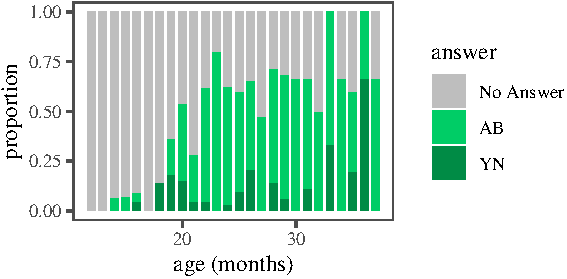
\includegraphics{figs/answerPlot-1} 

}

\caption{Left: Monthly proportions of children's yes/no (YN) and alternative (AB) answers to questions with \textit{or}. Right: Monthly proportions of children's appropriate answers to questions with \textit{or}.}\label{fig:answerPlot}
\end{figure}

\begin{figure}[tb]

{\centering 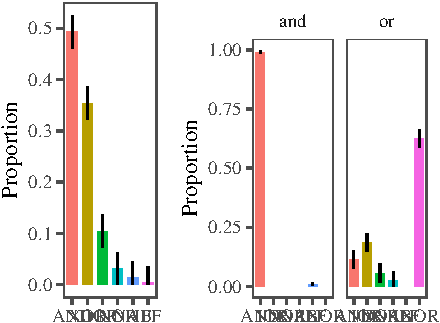
\includegraphics{figs/interpretationPlot-1} 

}

\caption{Left: Connective interpretations in child-directed speech. Right: Connective interpretations broken down by lexical items \textit{and} (conjunction) and \textit{or} (disjunction).}\label{fig:interpretationPlot}
\end{figure}

First, we look at our dependent variable, namely \enquote{connective interpretations}. Figure \ref{fig:interpretationPlot} (Left) shows the overall distribution of the connective interpretations in child-directed speech regardless of the connective word. The most common interpretation was conjunction (AND, 55\%) followed by exclusive disjunction (XOR, 31\%). Figure \ref{fig:interpretationPlot} (Right) shows the distribution of connective interpretations broken down by the connective word used: \emph{and} vs. \emph{or}\footnote{All the confidence intervals shown in the plots for this section are simultaneous multinomial confidence intervals computed using the Sison and Glaz (1995) method.}. Almost all instances of the connective \emph{and}, were interpreted as conjunction (AND). There were also a small number of NAND interpretations (e.g. \enquote{don't swing that in the house and hit things with it}) and IFF interpretations (e.g. \enquote{come here and I'll show you}) in our sample. For the connective \emph{or}, the most frequent interpretation was exclusive disjunction (XOR, 62\%) followed by inclusive disjunction (IOR, 18\%) and conjunction (AND, 11\%). There were also a small number of NOR (e.g. \enquote{you never say goodbye or thank you}) and NAB interpretations (e.g. \enquote{those screws, or rather, those nuts}). Overall, these results are consistent with the findings of Morris (2008) who concluded that exclusive disjunction is the most common interpretation of \emph{or}. Therefore, by simply associating the most common interpretations with the connective words, a learner is expected to learn \emph{and} as conjunction, and \emph{or} as exclusive disjunction (Crain, 2012; Morris, 2008).

\begin{figure}[tb]

{\centering 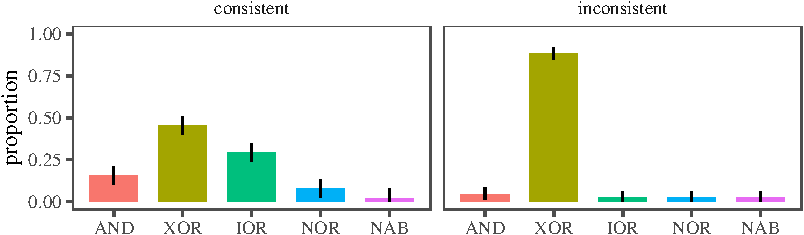
\includegraphics{figs/consistencyPlot-1} 

}

\caption{Interpretations of disjunction with consistent vs. inconsistent disjuncts.}\label{fig:consistencyPlot}
\end{figure}

However, the learning outcome might be different if factors other than the connective word are also considered. In what follows, we investigate how different annotation categories introduced earlier correlate with the interpretations of \emph{or}. We set \emph{and} aside because it was almost always interpreted as conjunction (AND). Figure \ref{fig:consistencyPlot} shows the proportions of connective interpretations in disjunctions with consistent vs.~inconsistent disjuncts. When the disjuncts were consistent (i.e.~could be true at the same time), the interpretation could be exclusive (XOR), inclusive (IOR), or conjunctive (AND). When the disjuncts were inconsistent, a disjunction almost always received an exclusive (XOR) interpretation. This suggests that the exclusive interpretation of a disjunction often stems from the inconsistent or contradictory nature of the disjuncts themselves\footnote{It should be noted here that in all \emph{and}-examples, the disjuncts were consistent. This is not surprising given that inconsistent meanings with \emph{and} result in a contradiction. The only exception to this was one example where the mother was mentioning two words as antonyms: \enquote{short and tall}. This example is quite different from the normal utterances given that it is meta-linguistic and list words rather than asserting the content of the words.}.

\begin{figure}[tb]

{\centering 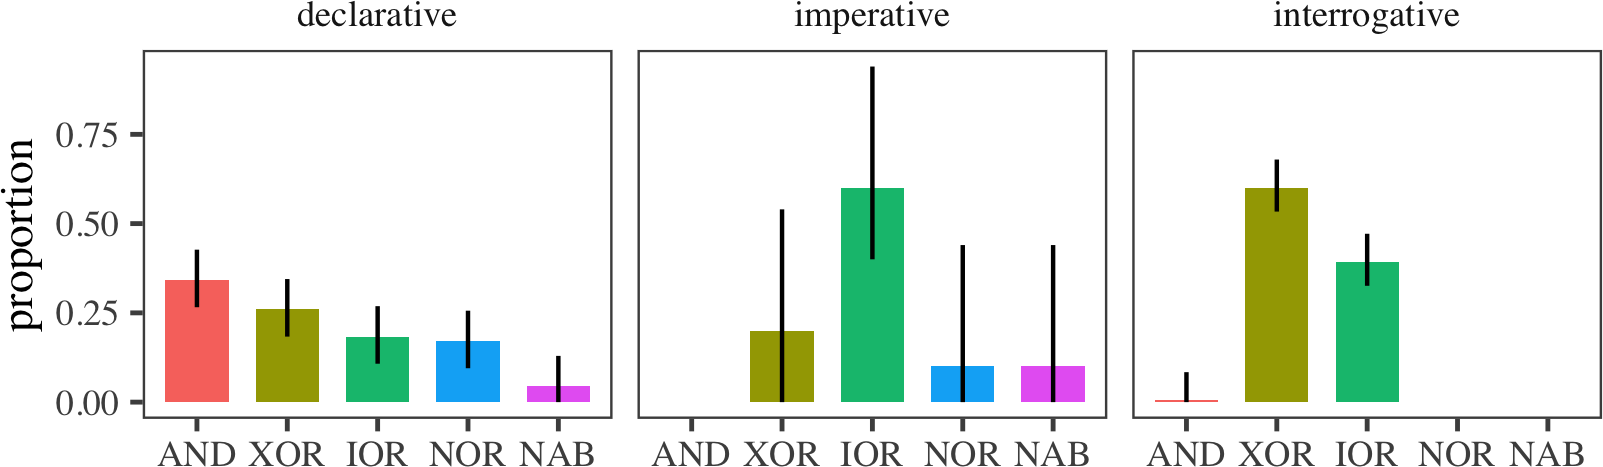
\includegraphics{figs/utterancePlot-1} 

}

\caption{Interpretations of disjunction with consistent disjuncts in interrogative, imperative, and declarative utterances.}\label{fig:utterancePlot}
\end{figure}

Next we focus on cases of disjunction with consistent disjuncts. Figure \ref{fig:utterancePlot} shows their interpretations in declarative, interrogative, and imperative sentences. Interrogatives selected for exclusive and inclusive interpretations. Imperatives were more likely to be interpreted as inclusive (IOR), but declaratives could receive almost any interpretation: conjunctive (AND), exclusive (XOR), inclusive (IOR), or even that \enquote{neither} disjunct was true (NOR). A common example of inclusive imperatives was invitation to action such as \enquote{Have some food or drink!}. Such invitational imperatives seem to convey inclusivity (IOR) systematically. They are often used to give the addressee full permission with respect to both alternatives. It can in fact be odd to use them to imply exclusivity (e.g. \enquote{Have some food or drink, but not both!}), and they are not conjunctive either, i.e inviting the addressee to do both actions (e.g. \enquote{Have some food, and have some drink!}).

\begin{figure}[tb]

{\centering 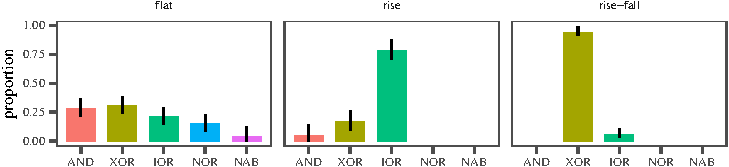
\includegraphics{figs/intonationPlot-1} 

}

\caption{Interpretations of disjunction with consistent disjuncts and flat, rising, or rise-fall intonation.}\label{fig:intonationPlot}
\end{figure}

While interrogatives selected for exclusive and inclusive interpretations, their intonation could distinguish between these two readings. Figure \ref{fig:intonationPlot} shows the interpretations of consistent disjunction in three intonational contours: flat, rise, and rise-fall. The rise and rise-fall contours are typical of interrogatives. The results show that, a disjunction with a rise-fall intonation is most likely interpreted as exclusive (XOR). If the intonation is rising, a disjunction is most likely inclusive (IOR). Finally, a disjunction with a flat intonation (typical of declaratives and imperatives) could be interpreted as exclusive (XOR), conjunctive (AND), inclusive (IOR), or neither (NOR). These results replicate Pruitt and Roelofsen (2013)'s experimental findings on the role of intonation in the interpretation of polar and alternative questions.

\begin{figure}[tb]

{\centering 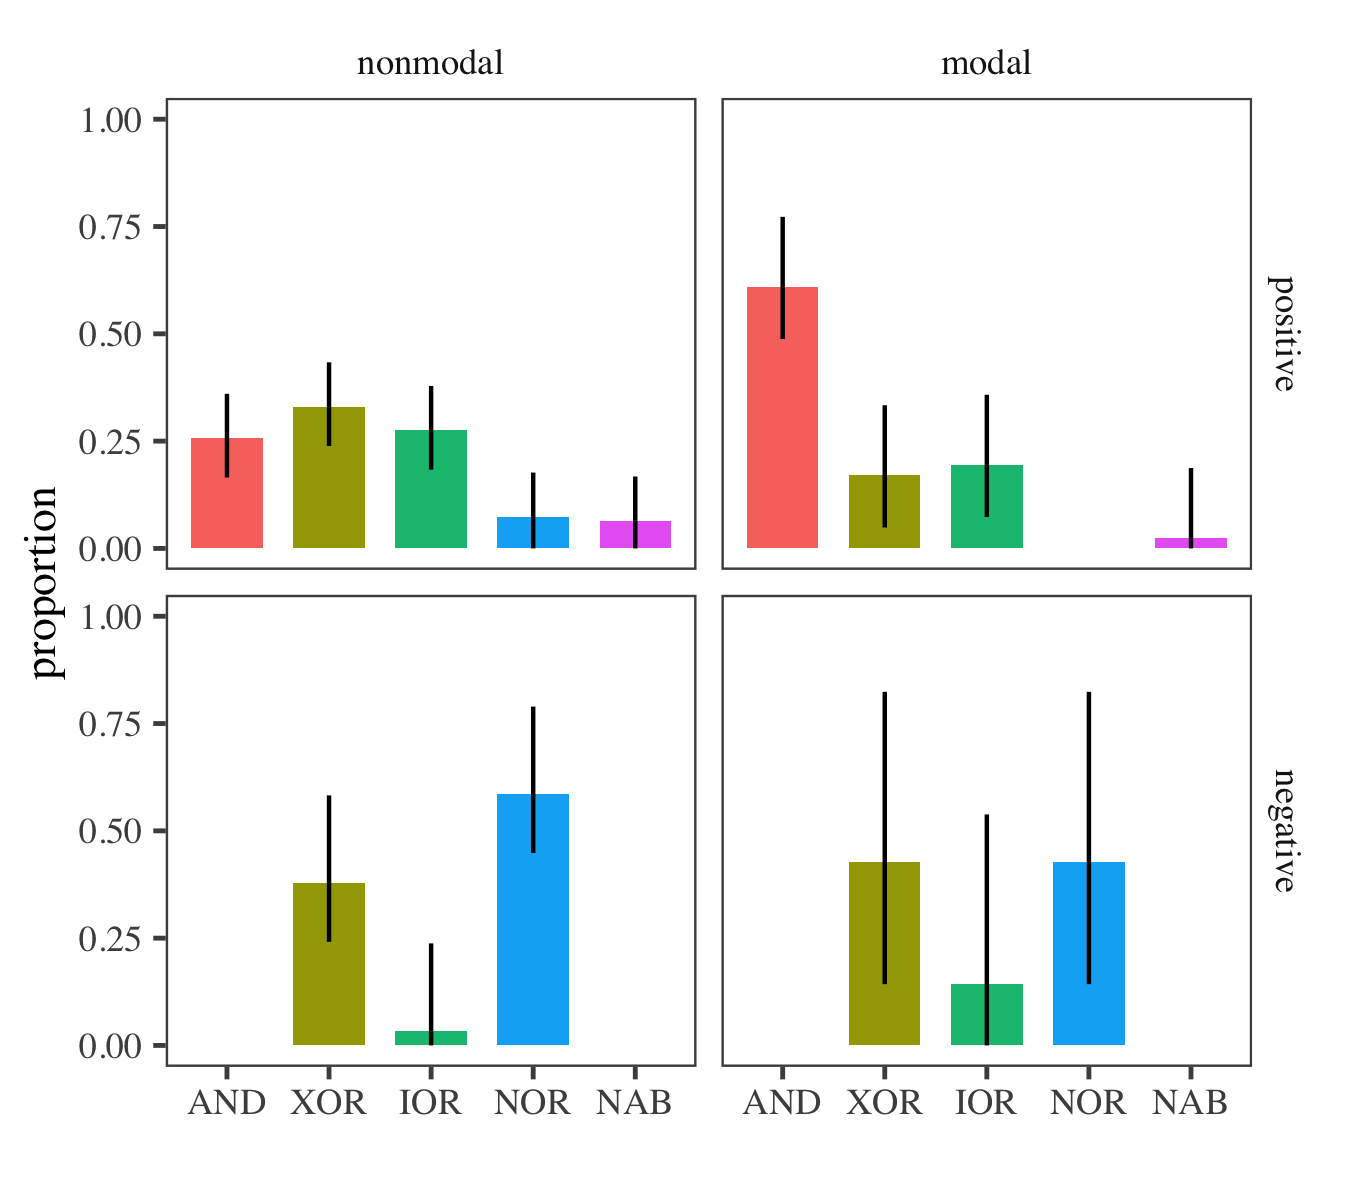
\includegraphics{figs/negModalPlot-1} 

}

\caption{Distribution of connective interpretations for consistent disjuncts with flat intonation.}\label{fig:negModalPlot}
\end{figure}

Next we focus on consistent disjunctions with flat intonation. Figure \ref{fig:negModalPlot} breaks down the interpretations based on whether the utterance contained negation or modals. The results show that in the presence of a modal such as \emph{can} or \emph{maybe}, it was more likely for a disjunction to have a conjunctive interpretation. This is consistent with the literature on free-choice inferences in formal semantics and pragmatics (Kamp, 1973), which shows statements such as \enquote{you can have tea or coffee} is interpreted conjunctively as \enquote{you can have tea \emph{and} you can have coffee}. When the utterance contained a negation, the disjunction could be interpreted as exclusive (XOR) or neither (NOR). These two interpretations correspond to the scope relations between negation and disjunction. If negation scopes above disjunction, we get a neither (NOR) interpretation (e.g. \enquote{I do not eat cauliflower, cabbage or baked beans.}) But if disjunction scopes above negation, the likely interpretation is exclusive (e.g.~don't throw it at the camera or you're going in the house.) These results also suggest that a learner who tracks co-occurences of \emph{or} with negative morphemes can potentially learn about the scope interaction of disjunction and negative particles in their native language.

\begin{figure}[tb]

{\centering 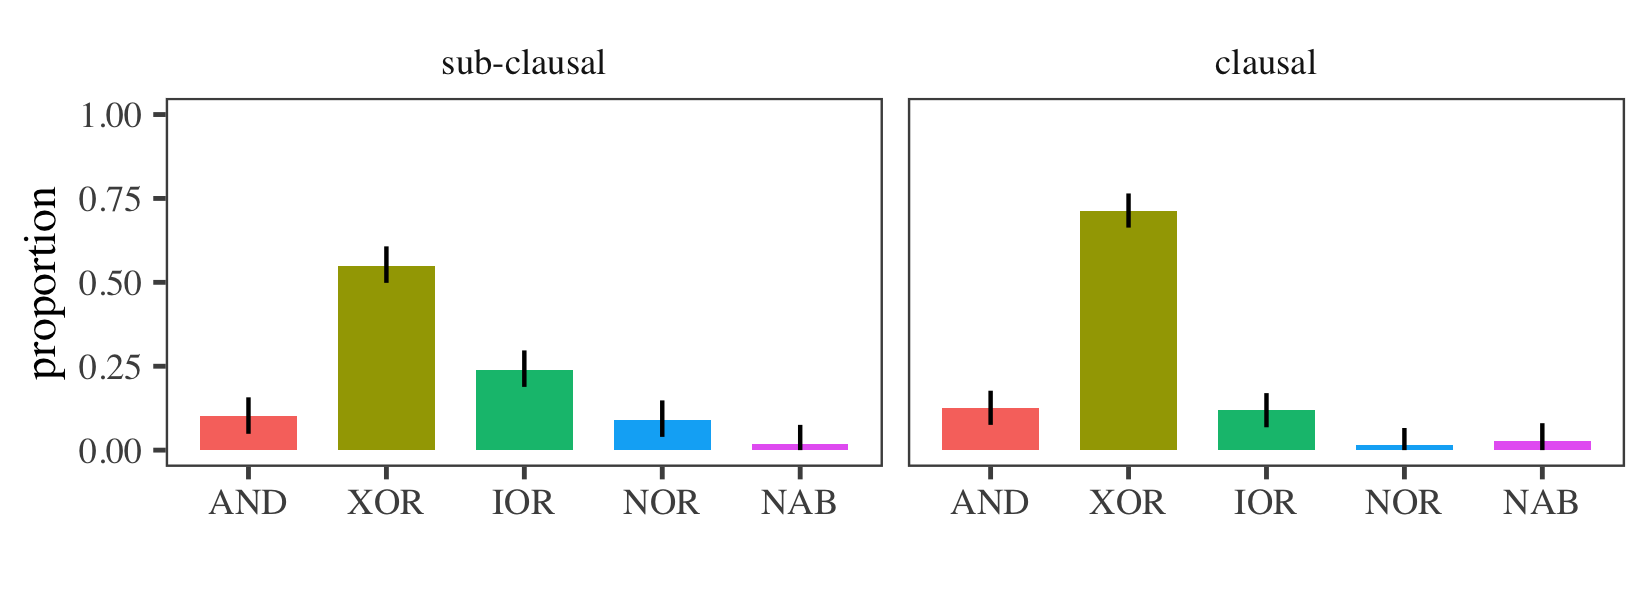
\includegraphics{figs/syntaxPlot-1} 

}

\caption{Top: Interpretations of clausal vs. sub-clausal disjunction. Down: Interpretations of clausal vs. sub-clausal disjunction in declaratives with consistent disjuncts.}\label{fig:syntaxPlot}
\end{figure}

Finally, we visit the last two remaining categories: syntactic level and communicative functions. For these categories, we show connective interpretations over all instances of disjunction. Figure \ref{fig:syntaxPlot} shows connective interpretations, broken down by syntactic level. The results suggest a possible small effect of clausal level disjuncts. Disjunctions were more likely to be interpreted as exclusive if their disjuncts were clauses or verbs rather than nominals, adjectives, or prepositions (all sub-clausal units). As explained before, the intuition is that a sentences such as \enquote{They had tea or coffee} is less likely to be exclusive than \enquote{they had tea or they had coffee} However, our understanding is that compared to other factors such as intonation and consistency, the effect of syntactic level was very small. As we shall see in Study 3, a computational learning model did not find syntactic level to be of much use for classifying instances of disjunction as exclusive, above and beyond what other annotation categories offered.

\begin{figure}[tb]

{\centering 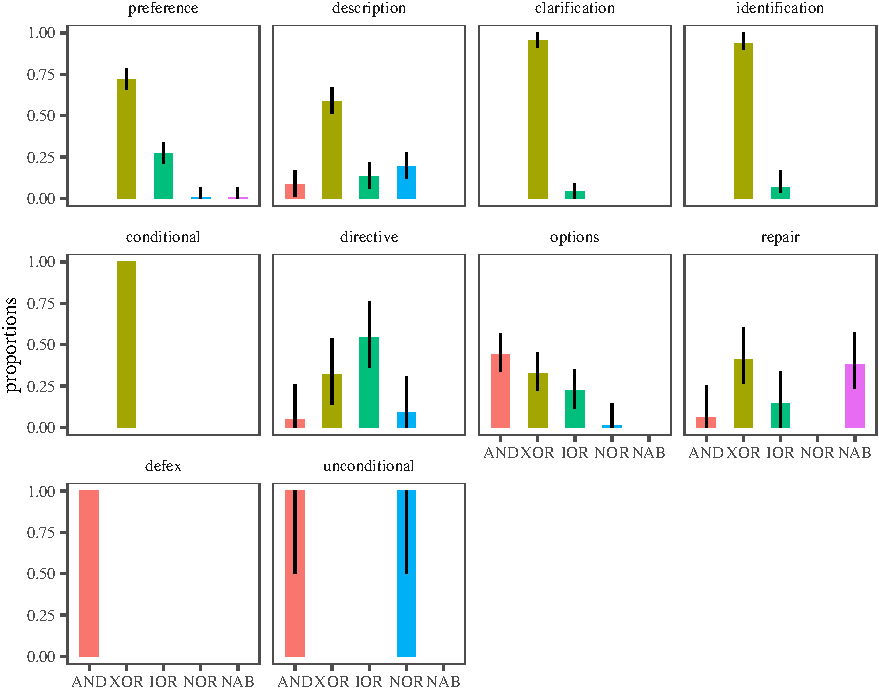
\includegraphics{figs/speechActPlot-1} 

}

\caption{Interpretations of disjunction in different communicative functions.}\label{fig:speechActPlot}
\end{figure}

Figure \ref{fig:speechActPlot} shows connective interpretations in the 10 different communicative functions we defined. The results show that certain functions increase the likelihood of some connective interpretations. An exclusive interpretation (XOR) is common in acts of clarification, identification, stating/asking preferences, stating/asking about a description, or making a conditional statements. These results are consistent with expectations on the communicative intentions that these utterances carry. In clarifications, the speaker needs to know which of two alternatives the other party meant. Similarly in identifications, speaker needs to know which category does a referent belongs to. In preferences, parents seek to know which of two alternatives the child wants. Even though descriptions could be either inclusive or exclusive, in the current sample, most descriptions were questions about the state of affairs and required the child to provide one of the alternatives as the answer. In conditionals such as \enquote{come here or you are grounded}, the point of the threat is that only one disjunct can be true: either \enquote{you come and you are not grounded} or \enquote{you don't come and you are grounded}.

Repairs often received an exclusive (XOR) or a second-disjunct-true (NAB) interpretation. This is expected given that in repairs the speaker intends to say that the first disjunct is incorrect or inaccurate. Unconditionals and definitions/examples always had a conjunctive (AND) interpretation. Again, this is to be expected. In such cases the speaker intends to communicate that all options apply. If the mother says that \enquote{cats are animals like lions or tigers}, she intends to say that both lions and tigers are cats, and not one or the other. Interestingly, in some cases, \emph{or} is replaceable by \emph{and}: \enquote{cats are animals like lions and tigers}. In unconditionals, the speaker communicates that in both alternatives, a certain proposition holds. For example, if the mother says \enquote{ready or not, here I come!}, she communicates that \enquote{I come} is true in both cases where \enquote{you are ready} and \enquote{you are not ready}.

Options were often interpreted either as conjunctive (AND) or inclusive (IOR). The category \enquote{options} contained examples of free-choice inferences such as \enquote{you could drink orange juice or apple juice}. This study found free-choice examples to be more common in child-directed speech than the current literature on the acquisition of disjunction assumes. Finally, directives received either an IOR or XOR interpretation. It is important to note here that the most common communicative function in the data were preferences and descriptions. Other communicative functions such as unconditionals or options were fairly rare. Despite their infrequent appearance, these constructions must be learned by children at some point, since almost all adults know how to interpret them.

\hypertarget{conclusion}{%
\subsection{Conclusion}\label{conclusion}}

This study focused on the interpretations that connectives \emph{and} and \emph{or} recieve in child-directed speech. It also investigated some candidate cues that can help children's learning of these interpretations. The study selected 1000 examples of \emph{and} and \emph{or} in child-directed speech, annotated for their truth-conditional interpretation, as well as six candidate cues: (1) Conceptual Consistency (2) Utterance Type; (3) Intonation; (4) Presence of negative or modal morphemes (5) Syntactic Level; and (6) Communicative Function. Like Morris (2008), this study found that the most common interpretations of \emph{and} and \emph{or} are conjunction (AND) and exclusive disjunction (XOR) respectively. Therefore, relying only on connective word forms, a learner should expect \emph{and} to be a conjunction and \emph{or} exclusive disjunction.

However, the study also found that the most likely interpretation of a disjunction depended on the cues that accompanied it in context. A disjunction was most likely exclusive if the alternatives were inconsistent (i.e.~contradictory). A disjunction with consistent alternatives was either inclusive or exclusive if it appeared in a question. Within questions, a disjunction was most likely exclusive if its intonation was \enquote{rise-fall}, and inclusive if it was \enquote{rising}. Among declaratives and imperatives with \enquote{flat} intonations, a disjunction was interpreated most liklely as AND if there was a modal, and NOR or XOR if there was negation present in the utterance. Finallly, in the absence of all these cues, a disjunction was more likely to be non-exclusive (IOR + AND) than exclusive (XOR). These results suggest that a learner can potentially use these cues to predict the intended interpretation of a connective in utterance context. In the next study, we use a computational learning model to formalize this account.

\hypertarget{study-3-computational-modeling-using-decision-trees}{%
\section{Study 3: Computational Modeling Using Decision Trees}\label{study-3-computational-modeling-using-decision-trees}}

A decision tree is a classification model structured as a hierarchical tree with an initial node, called the root, that branches into more nodes until it reaches the leaves (Breiman, 2017). Each node represents a test on a feature, each branch represents an outcome of the test, and each leaf represents a classification label. Using a decision tree, observations can be classified or labeled based on a set of features. Decision trees have at least three advantages for modeling cue-based accounts of semantic acquisition. First, the features used in decision trees for classification can be the cues that help the acquisition and interpretation of a word or an utterance. Second, unlike many other machine learning techniques, decision trees result in models that are interpretable. Third, the order of decisions or features used for classification is determined based on information gain. Features that appear higher (earlier) in the tree are more informative and helpful for classification. Therefore, decision trees can help us understand which cues are more helpful for the acquisition and interpretation of words.

<<<<<<< HEAD
Decision tree learning is the construction of a decision tree from labeled training data. This section applies decision tree learning to the annotated data of Study 2 by constructing random forests (Breiman, 2001; Ho, 1995). In random forest classification, multiple decision trees are constructed on subsets of the data, and each tree predicts a classification. The ultimate outcome is a majority vote of each trees classification. Since decision trees tend to overfit data, random forests control for overfitting by building more trees and averaging their results. (Breiman, 2001) Next section discusses the methods used in constrcting the random forests for interpreting connectives \emph{or}/\emph{and}.
=======
Decision tree learning is the construction of a decision tree from labeled training data. This section applies decision tree learning to the annotated data of Study 2 by constructing random forests (Breiman, 2001; Ho, 1995). In random forest classification, multiple decision trees are constructed on subsets of the data, and each tree predicts a classification. The ultimate outcome is a majority vote of each tree's classification. Since decision trees tend to overfit data, random forests control for overfitting by building more trees and averaging their results. \textbf{(Citation)} In the context of semantic acquisition, the random forest can represent hypothetical variability in the learners. The next section discusses the methods used in constrcting the random forests for interpreting the connectives \emph{or} and \emph{and}.
>>>>>>> master

\hypertarget{methods-2}{%
\subsection{Methods}\label{methods-2}}

<<<<<<< HEAD
The random forest models were constructed using python's Sci-kit Learn package (Pedregosa et al., 2011). The annotated data had a feature array (see Study 2) and a connective interpretation label for each connective use. Connective interpretations included exclusive (XOR), inclusive (IOR), conjunctive (AND), negative inclusive (NOR), and NPQ which states that only the second proposition is true. The features (or \enquote{cues}) included all other annotation categories: intonation, consistency, syntactic level, utterance type, and communicative function. All models were trained with stratified 10-Fold cross-validation to reduce overfitting. Stratified cross-validation maintains the distribution of the initial data in the random sampling to build cross validated models. Maintaining the data distribution ensures a more realistic learning environment for the forests. Tree success was measured with F1-Score, harmonic average of precision and recall.

First a grid search was run on the hyperparamter space to establish the number of trees in each forest and the maximum tree depth allowable. The grid search creates a grid of all combinations of forest size and tree depth and then trains each forest from this grid on the data (Pedregosa et al., 2011). The forests with the best F1-score and lowest size/depth are reported. The default number of trees for the forests was set to 20, with a max depth of eight and a minimum impurity decrease of 0. Impurity was measured with gini impurity, which states the odds that a random member of the subset would be mislabled if it were randomly labeled according to the distribution of labels in the subset. \textbf{(Citation)}

Decision trees were fit with high and low minimum gini decrease values. High minimum gini decrease results in a tree that does not use any features for branching. Such a tree represents the baseline or frequentist approach to mapping that directly maps a word to its most frequent interpretation. Low minimum gini decrease allows for a less conservative tree that uses multiple cues/features to predict the interpretation of a disjunction. Such a tree represents the cue-based context-sensitive account of word learning discussed in the previous section.
=======
The random forest models were constructed using python's Sci-kit Learn package (Pedregosa et al., 2011). The annotated data had a feature array and a connective interpretation label for each connective use. Connective interpretations included exclusive (XOR), inclusive (IOR), conjunctive (AND), negative inclusive (NOR), and NPQ which states that only the second proposition is true. The features or cues used included all other annotation categories: intonation, consistency, utterance type, syntactic level, negation, modals, and communicative function. All models were trained with stratified 10-Fold cross-validation to reduce overfitting. Stratified cross-validation maintains the distribution of the initial data in the random sampling to build cross validated models. Maintaining the data distribution ensures a more realistic learning environment for the forests. Tree success was measured with F1-Score, harmonic average of precision and recall (Rijsbergen, 1979).

First a grid search was run on the hyperparamter space to establish the number of trees in each forest and the maximum tree depth allowable. The grid search creates a grid of all combinations of forest size and tree depth and then trains each forest from this grid on the data. The forests with the best F1-score and lowest size/depth are reported. **(Citation*)** The default number of trees for the forests was set to 20, with a max depth of eight and a minimum impurity decrease of 0. Impurity was measured with gini impurity, which states the odds that a random member of the subset would be mislabled if it were randomly labeled according to the distribution of labels in the subset. (Gini, 1912).

Decision trees were fit with high and low minimum-gini-decrease values. High minimum-gini-decrease results in a tree that does not use any features for branching. Such a tree represents the baseline or traditional approach to mapping that directly maps a word to its most likely interpretation. Low minimum-gini-decrease allows for a less conservative tree that uses multiple cues or features to predict the interpretation of a disjunction. Such a tree represents the cue-based context-sensitive account of word learning.
>>>>>>> master

\hypertarget{results-1}{%
\subsection{Results}\label{results-1}}

<<<<<<< HEAD
We first present the results of the random forests in a binary classification task. The models were trained to classify exclusive (XOR, NPQ) and inclusive (AND, IOR, NOR) interpretations of disjunction. For visualization of trees, we selected the highest performing tree in the forest by testing each tree and selecting for highest F1 score. While the forests performance is not identical to the highest performing tree, the best tree gives an illustrative example of how the tree performs.

Figure \ref{fig:binaryBaseline} shows the best performing decision tree with high minimum gini decrease. As expected, a learner that does not use any cues would interpret \emph{or} as exclusive all the time. This is the baseline model. Figure \ref{fig:binaryCueBased} shows the best performing decision tree with low minimum gini decrease. The tree has learned to use intonation and consistency to classify disjunctions as exclusive or inclusive. As expected, if the intonation is rise-fall or the disjuncts are inconsistent, the interpretation is exclusive. Otherwise, the disjunction is classified as inclusive.
=======
We first present the results of the random forests in the binary classification task. The models were trained to classify exclusivity, e.i. whether an interpretation was exclusive or not. For visualization of trees, we selected the highest performing tree in the forest by testing each tree and selecting for highest F1 score. While the forests performance is not identical to the highest performing tree, the best tree gives an illustrative example of successful learning from data. Figure \ref{fig:binaryBaseline} shows the best performing decision tree with high minimum gini decrease. As expected, a learner that does not use any cues would interpret \emph{or} as exclusive all the time. This is the baseline model. Figure \ref{fig:binaryCueBased} shows the best performing decision tree with low minimum gini decrease. The tree has learned to use intonation and consistency to classify disjunctions as exclusive or inclusive. As expected, if the intonation is rise-fall or the disjuncts are inconsistent, the interpretation is exclusive. Otherwise, the disjunction is classified as not exclusive.
>>>>>>> master

\begin{figure}
\centering
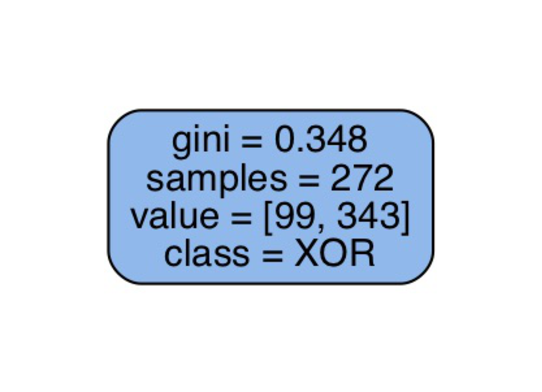
\includegraphics{figs/binaryBaseline-1.pdf}
\caption{\label{fig:binaryBaseline}(A) The structure for the baseline (highest gini threshold, 0.2) decision tree trained on examples with exclusive (EX) and non-exclusive (IN) interpretations. (B) The structure for the cue-based decision tree (low gini threshold of 0.01). The average F1 score with 95\% confidence intervals as a function of the number of training examples in the baseline and cue-based model when treating as positive (C) EX and (D) IN respectively.}
\end{figure}

\begin{figure}
\centering
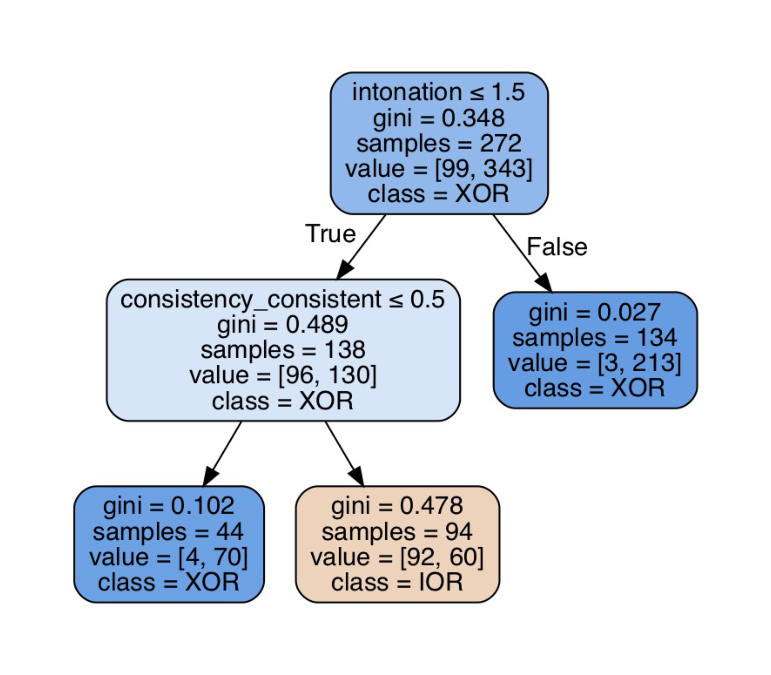
\includegraphics{figs/binaryCueBased-1.pdf}
<<<<<<< HEAD
\caption{\label{fig:binaryCueBased}Cue-based tree grown with minimum impurity decrease of 0.01. The tree classifies examples of disjunction with rise-fall intonation as exclusive (intonation \textgreater{} 1.5). If the intonation is not rise-fall but the disjuncts are inconsistent (consistency \textless{} 0.5), then the disjunction is still classified as exclusive. However, if neither of these two hold, the disjunction is classified as inclusive.}
\end{figure}

Figure \ref{fig:XorBinary} shows the average F1 scores of the baseline and cue-based models in classifying exclusive examples as the number of training examples increases. The models perform similarly, but the cue-based model performs slightly better (no significant difference). The real difference between the baseline model and the cue-based model is in their performance on inclusive examples. Figure \ref{fig:IorBinary} shows the F1 score of the forests as a function of the training size in classifying inclusive examples. As expected, the baseline model performs very poorly while the cue-based model improves with more examples and performs significantly better than the baseline tree.

\begin{figure}
\centering
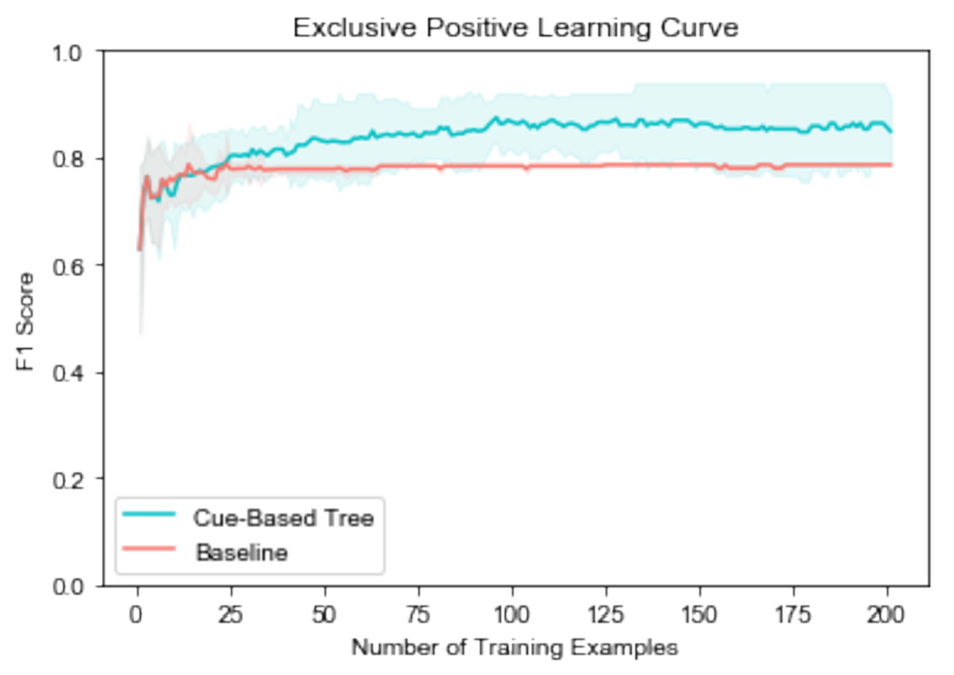
\includegraphics{figs/XorBinary-1.pdf}
\caption{\label{fig:XorBinary}The average F1 score for class XOR (exclusive) as a function of the number of training examples in the baseline and cue-based models. The colored shades show the 95\% confidence intervals.}
=======
\caption{\label{fig:binaryCueBased}(A) The structure for the baseline (highest gini threshold, 0.2) decision tree trained on examples with XOR, IOR, AND, and NOR interpretations. (B) The structure for the cue-based decision tree (low gini threshold of 0.01). The average F1 score with 95\% confidence intervals as a function of the number of training examples in the baseline and cue-based model when treating as positive (C) AND, (D) XOR, (E) IOR, (F) NOR respectively.}
>>>>>>> master
\end{figure}

Figure \ref{fig:XorBinary} shows the average F1 scores of the baseline and cue-based models in classifying exclusive examples as the number of training examples increases. The models perform similarly, but the cue-based model performs slightly better (no significant difference). The real difference between the baseline model and the cue-based model is in their performance on inclusive examples. Figure \ref{fig:IorBinary} shows the F1 score of the forests as a function of the training size in classifying inclusive examples. As expected, the baseline model performs very poorly while the cue-based model improves with more examples and performs significantly better than the baseline tree.

Next, we use decision tree learning in a ternary classification task. The model uses features to interpret a coordination with \emph{and} and \emph{or} as inclusive (IOR), exclusive (XOR), or conjunctive (AND). Figure \ref{fig:ternaryBaseline} shows the baseline decision tree with high minimum gini decrease, which only uses the presence of the words \emph{or}/\emph{and} to interpret conjunction and disjunction. As expected, the tree interprets a coordination with \emph{and} as a conjunction and one with \emph{or} as exclusive disjunction. Figure \ref{fig:ternaryCueBased} shows the cue-based decision tree with low minimum gini decrease. In addition to the presence of \emph{and} and \emph{or}, the tree uses intonation, consistency, communicative function, and sentence type to distinguish exclusive, inclusive, and conjunctive uses of disjunction. In short, a disjunction that is rise-fall, inconsistent, or has a conditional communicative function is classified as exclusive. Otherwise the disjunction is classified as inclusive. The tree also finds conjunctive interpretations of disjunction more likely in declarative sentences than interrogatives.

<<<<<<< HEAD
\begin{figure}
\centering
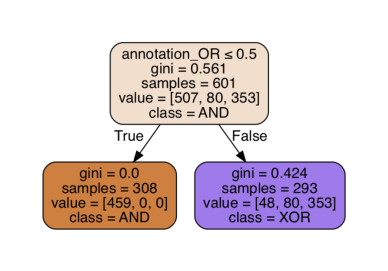
\includegraphics{figs/ternaryBaseline-1.pdf}
\caption{\label{fig:ternaryBaseline}The baseline tree grown on conjunctions and disjunctions with minimum impurity decrease of 0.2. The tree uses the words \textit{and/or} and classifies them as conjunction and exclusive disjunction respectively.}
\end{figure}

\begin{figure}
\centering
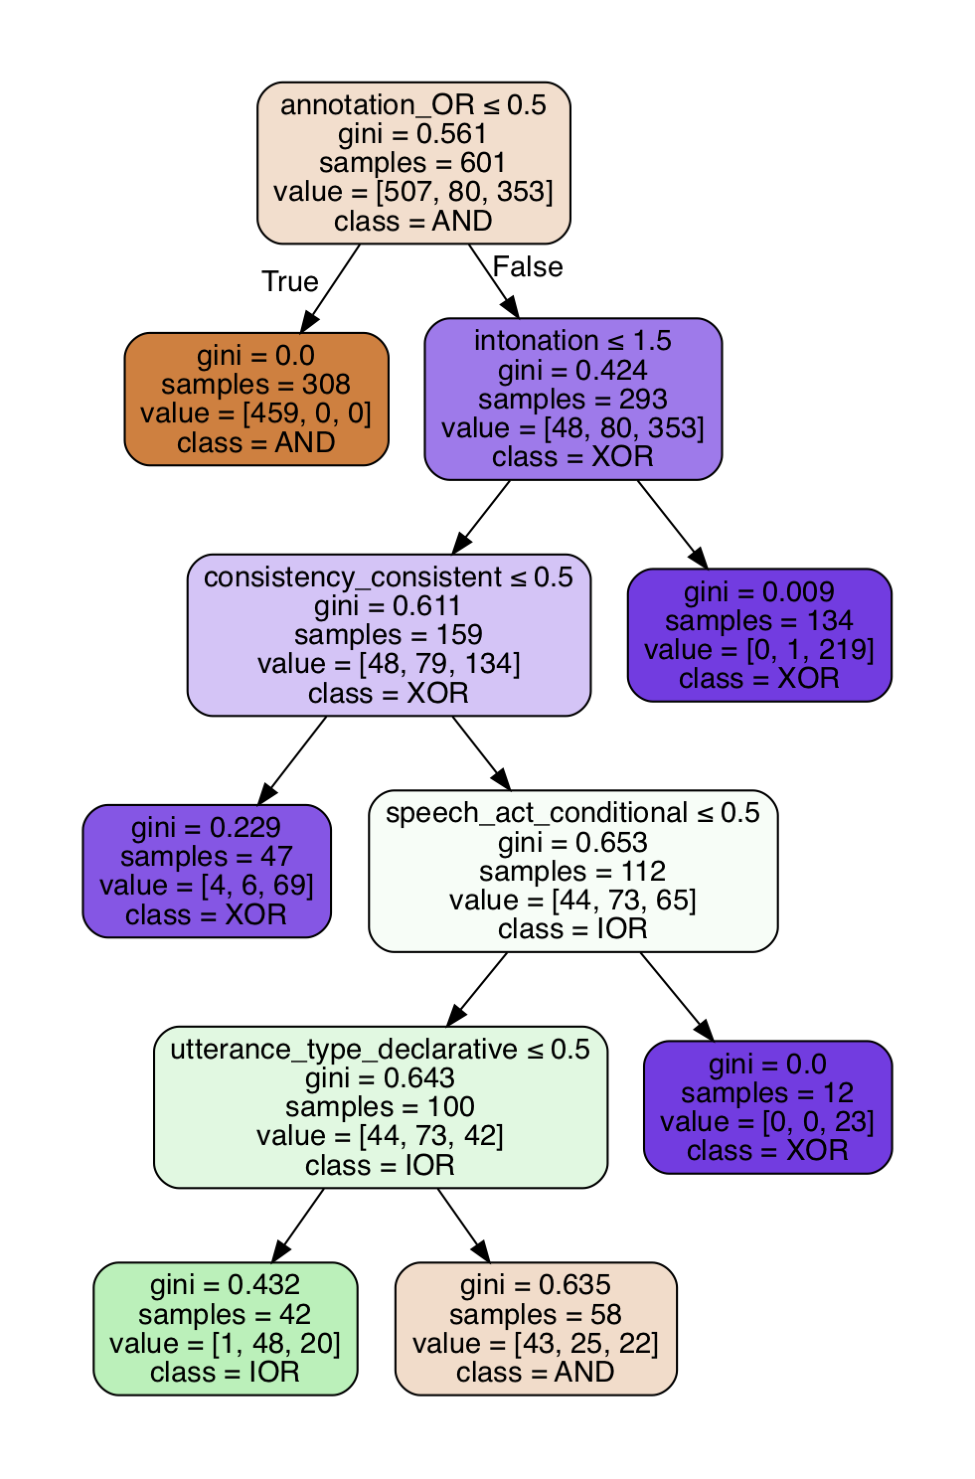
\includegraphics{figs/ternaryCueBased-1.pdf}
\caption{\label{fig:ternaryCueBased}The cue-based tree grown on conjunctions and disjunctions with minimum impurity decrease of 0.01. After using the words \textit{and/or}, the tree uses intonation, consistency, and the conditional communicative function to classify a large number of exclusive cases. Then it uses utterance type (interrogative) to label inclusive cases.}
\end{figure}

Figure \ref{fig:ANDintermediate} shows the average F1 score of the conjunctive interpretations (AND) for the baseline and the cue-based models. Since the vast majority of the conjunctive interpretations are predicted by the presence of the word \emph{and}, the baseline and cue-based models show similar performances. Setting aside conjunction examples, Figure \ref{fig:ANDintermediateDis} shows the average F1 score of the AND interpretation of disjunction only. Here we see that the cue-based model performs better than the default model in predictiving conjunctive interpretations of OR utterances. The informal analysis of the trees suggest that the model does this by using the \enquote{speech act} cue. Figure \ref{fig:XORintermediate} shows the average F1-score of the exclusive interpretations (XOR) for the baseline and the cue-based models. The cue-based model does slightly better than the baseline model. As before, the most important improvement comes in identifying inclusive examples. Figure \ref{fig:IORintermediate} shows the average F1-score of the inclusive interpretations (IOR) for both baseline and cue-based models. The baseline model performs very poorly while the cue-based model is capable of classifying inclusive examples as well.
=======
Figure \ref{fig:ANDintermediate} shows the average F1 score of the conjunctive interpretations (AND) for the baseline and the cue-based models. Since the vast majority of the conjunctive interpretations are predicted by the presence of the word \emph{and}, the baseline and cue-based models show similar performances. Setting aside conjunction examples, Figure \ref{fig:ANDintermediateDis} shows the average F1 score of the AND interpretation of disjunction only. Here we see that the cue-based model performs better than the default model in guessing conjunctive interpretations of disjunction. The informal analysis of the trees suggest that the model does this by using the \enquote{speech act} cue. Figure \ref{fig:XORintermediate} shows the average F1-score of the exclusive interpretations (XOR) for the baseline and the cue-based models. The cue-based model does slightly better than the baseline model. As before, the most important improvement comes in identifying inclusive examples. Figure \ref{fig:IORintermediate} shows the average F1-score of the inclusive interpretations (IOR) for both baseline and cue-based models. The baseline model performs very poorly while the cue-based model is capable of classifying inclusive examples as well.
>>>>>>> master

Finally, we look at decision trees trained on the annotation data to predict all the interpretation classes for disjunction: AND, XOR, IOR, NOR, and NPQ. Figure \ref{fig:wholeBaseline} shows the baseline model that only uses the words \emph{and} and \emph{or} to classify. As expected, \emph{and} receives a conjunctive interpretation (AND) and \emph{or} receives an exclusive interpretation (XOR). Figure \ref{fig:wholeCueBased} shows the best example tree of the cue-based model. The leaves of the tree show that it recognizes exclusive, inclusive, conjunctive, and even negative inclusive (NOR) interpretations of disjunction. How does the tree achieve that? Like the baseline model, the tree first asks about the connective used: \emph{and} vs. \emph{or}. Then like the previous models, it asks about intonation and consistency. If the intonation is rise-fall, or the disjuncts are inconsistent, the interpretation is exclusive. Then it asks whether the sentence is an interrogative or a declarative. If interrogative, it guesses an inclusive interpretation. This basically covers questions with a rising intonation. Then the tree picks declarative examples that have conditional speech act (e.g. \enquote{give me the toy or you're grounded}) and labels them as exclusive. Finally, if negation is present in the sentence, the tree labels the disjunction as NOR.

Figures \ref{fig:ANDWhole}, \ref{fig:XORWhole}, and \ref{fig:IORWhole} show the average F1-scores for the conjunctive (AND), exclusive (XOR), and inclusive (IOR) interpretations as a function of training size. The results are similar to what wereported before with the ternary classification. While the cue-based model generally performs better than the baseline model, it shows substantial improvement in classifying inclusive cases. Figure \ref{fig:NORWhole} shows the average F1-score for the negative inclusive interpretation as a function of training size. Compared to the baseline model, the cue-based model shows a substantially better performance in classifying negative sentences. The success of the model in classifying negative inclusive examples (NOR) suggests that the cue-based model offers a promising approach for capturing the scope relation of operators such as negation and disjunction. Here, the model learns that when negation and disjunction are present, the sentence receives a negative inclusive (NOR) interpretation. In other words, the model has learned the narrow-scope interpretation of negation and disjunction from the input data. In a language where negation and disjunction receive an XOR interpretation (not A or not B), the cue-based model can learn the wide-scope interpretation of disjunction.

<<<<<<< HEAD
\begin{figure}
\centering
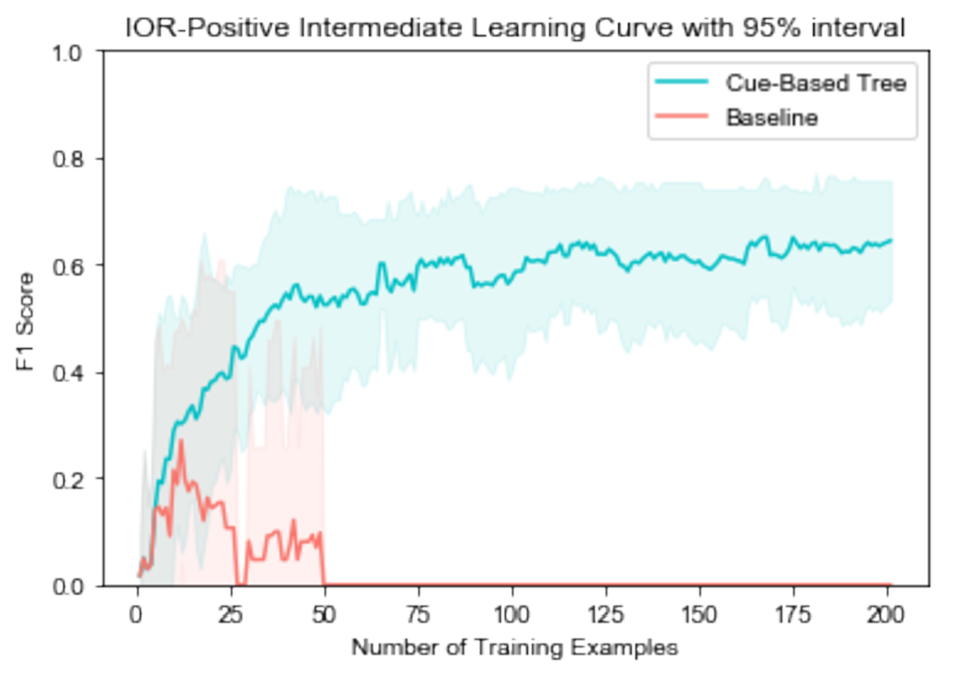
\includegraphics{figs/IORintermediate-1.pdf}
\caption{\label{fig:IORintermediate}The average F1 score for class IOR as a function of the number of training examples in the baseline and cue-based models. The colored shades show the 95\% confidence intervals.}
\end{figure}

Finally, we look at decision trees trained on the annotation data to predict all the interpretation classes for disjunction: AND, XOR, IOR, NOR, and NPQ. Figure \ref{fig:wholeBaseline} shows the baseline model that only uses the words \emph{and} and \emph{or} to classify. As expected, \emph{and} receives a conjunctive interpretation (AND) and \emph{or} receives an exclusive interpretation (XOR). Figure \ref{fig:wholeCueBased} shows the best example tree of the cue-based model. The leaves of the tree show that it recognizes exclusive, inclusive, conjunctive, and even negative inclusive (NOR) interpretations of disjunction. How does the tree achieve that? Like the baseline model, the tree first asks about the connective used: \emph{and} vs. \emph{or}. Then like the previous models, it asks about intonation and consistency. If the intonation is rise-fall, or the disjuncts are inconsistent, the interpretation is exclusive. Then it asks whether the sentence is an interrogative or a declarative. If interrogative, it guesses an inclusive interpretation. This basically covers questions with a rising intonation. Then the tree picks declarative examples that have conditional speech act (e.g. \enquote{give me the toy or you're grounded}) and labels them as exclusive. Finally, if negation is present in the sentence, the tree labels the disjunction as NOR.

\begin{figure}
\centering
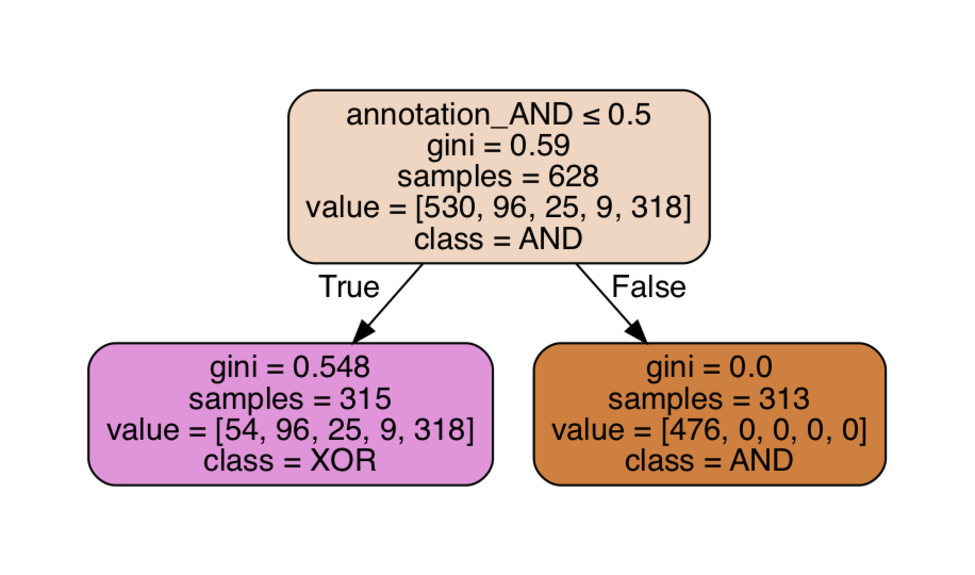
\includegraphics{figs/wholeBaseline-1.pdf}
\caption{\label{fig:wholeBaseline}The baseline tree grown on conjunctions and disjunctions with minimum impurity decrease of 0.2. The tree uses the words \textit{and/or} and classifies them as conjunction and exclusive disjunction.}
\end{figure}

\begin{figure}
\centering
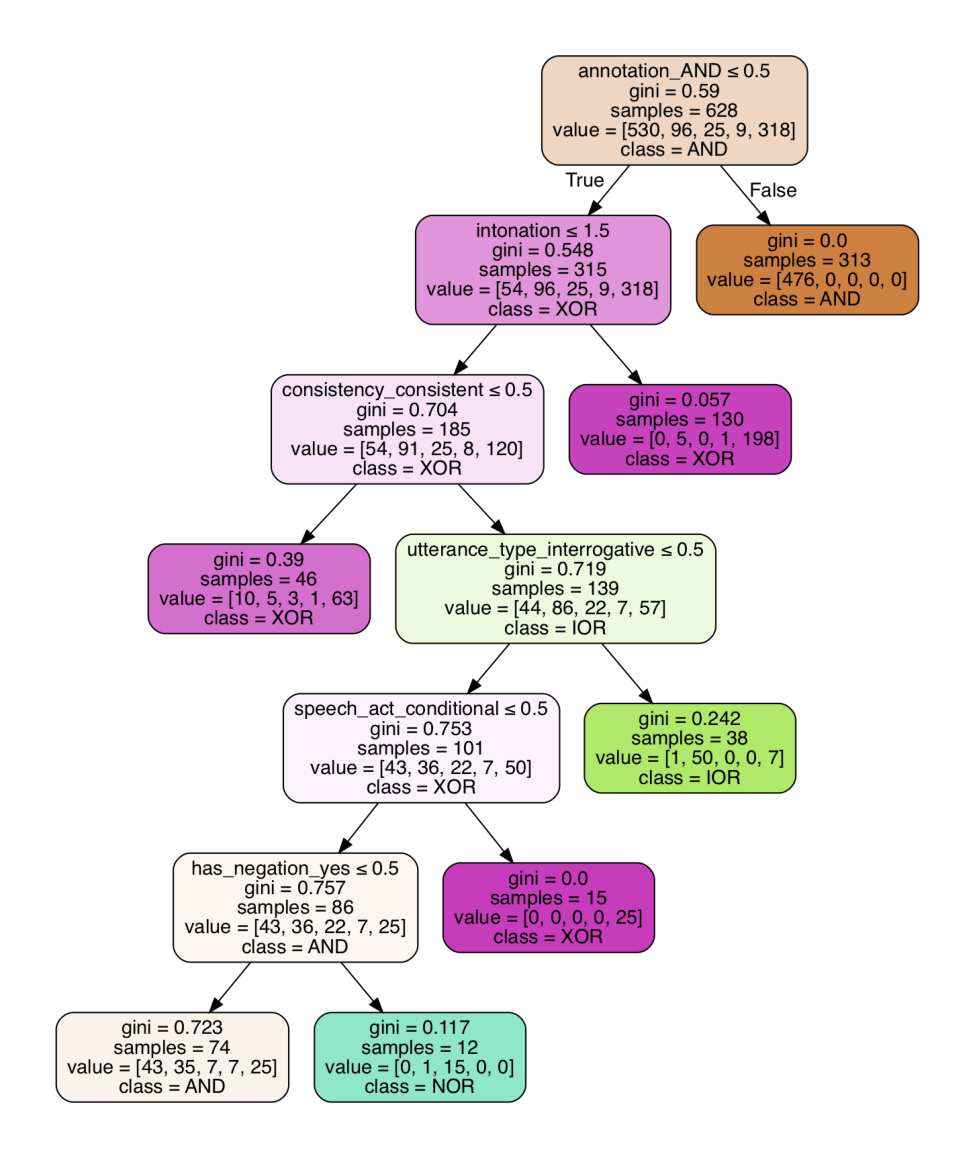
\includegraphics{figs/wholeCueBased-1.pdf}
\caption{\label{fig:wholeCueBased}The cue-based tree grown on conjunctions and disjunctions with minimum impurity decrease of 0.01. After using the words \textit{and/or}, the tree uses intonation and consistency to classify a large number of exclusive cases. Then it uses utterance type (interrogative) to label many inclusive cases, as well as the communicative function (conditional) to catch more exclusive examples. Finally, it asks whether the sentence has negation or not. If so, it classifies the negative inlusive examples as NOR.}
\end{figure}

Figures \ref{fig:ANDWhole}, \ref{fig:XORWhole}, and \ref{fig:IORWhole} show the average F1-scores for the conjunctive (AND), exclusive (XOR), and inclusive (IOR) interpretations as a function of training size. The results are similar to what we reported before with the ternary classification. While the cue-based model generally performs better than the baseline model, it shows substantial improvement in classifying inclusive cases.
=======
Finally, Figure \ref{fig:NPQWhole} shows the average F1 score for the class NPQ. This interpretation suggested that the first disjunct is false but the second true. It was seen in examples of repair most often and the most likely cue to it was also the communicative function or speech act of repair. The results show that even though there were improvements in the cue-based model, they were not stable as shown by the large confidence intervals. It is possible that with larger training samples, the cue-based model can reliably classify the NPQ interpretations as well.

\hypertarget{conclusion-1}{%
\subsection{Conclusion}\label{conclusion-1}}
>>>>>>> master

In this study, we used the annotation data from Study 2 to train and compare two random forest models, representing two accounts for the acquisition of disjunction. The first account was a baseline (context-independent) account in which words are isolated and directly mapped to their most likely meanings, disregarding available contextual cues. Random forest models with high minimum-gini-impurity-decrease represented this account. The second account was what we called the cue-based context-dependent mapping in which words are mapped to meanings using a set of cues available in the context. Random forest models with low minimum-gini-impurity-decrease represented this cue-based account. Comparison of the F1-Scores produced by models representing these two accounts showed that the cue-based models outperfromed the baseline models in every classification task. Most importantly, while the baseline models learned to always interpret a disjunction as exclusive, the cue-based models learned to interpret a disjunction as exclusive, inclusive, conjunctive, or negative inclusive (NOR), depending on the cues available in the input.

\hypertarget{general-discussion}{%
\section{General Discussion}\label{general-discussion}}

This paper presented three studies to support the claim that child-directed speech contains prosodic, conceptual, and linguistic cues that can aid the acquisition of linguistic disjunction. Study 1 presented the overall distribution of \emph{or} and \emph{and} in parents' and children's speech in CHILDES corpora. We found that children heared 1-2 examples of \emph{or} in every thousand words parents produced. Children started producing \emph{or} themselves between 18-30 months, and by 42 months they reached a rate of one \emph{or} per thousand words. Study 2 showed that as Morris (2008) had found, the most common interpretation of \emph{or} in child-directed speech is exclusive disjunction. However, we also found that exclusive interpretations were cued by prosodic and conceptual cues. In the absence of prosodic and conceptual cues to exclusivity, the interpretation of a disjunction was most likely non-exclusive. Finally, study 3 used decision-tree learning to show that a hypothetical learner can use prosodic, conceptual, and linguistic cues to predict the interpretation of a disjunction. It is importnat to note that while this study has shown the \textbf{potential utility} of conceptual, prosodic, and linguistic cues present in child-directed speech for the acquisition of disjunction, it has not actually established that children learning disjunction are sensitive to these cues, or that use them for learning. It is important for future experimental research to follow up and show that these cues are actually used by langauge learners in their acquisition of disjunction.

In what follows in this section, we place our findings and main claim in the bigger context of word learning. As we mentioned at the beginning, theories of word learning have been heavily influenced by Quine's Gavagai thought experiment; however, his specific views on word learning are not as widely discussed. Quine (1960) pinpointed several dimensions of word learning where theories can differ in their approach. First, Quine considered form-meaning mapping to occur at all levels of linguistic structure: words, phrases, and sentences. In other words, the learner could map any recognizable chunk or construction to candidate meanings, and store it in memory. This is in contrast to a view where only morphemes (smallest units) are mapped and stored, while larger units are derived compositionally. We call this dimension the \textbf{mapping unit}. Second, Quine considered three different ways of mapping words to meanings: isolated, context-dependent, and described. \enquote{Isolated mapping} refers to the case of hearing a word such as \enquote{chair}, \enquote{red}, or \enquote{run} and mapping it to the percieved object, property, or action isolated from its linguistic or communicative context. It is the classic Gavagai example. On the other hand, \enquote{context-dependent mapping} is learning a word \enquote{contextually, or by abstraction, as a fragment of sentences learned as wholes}. He suggested that \enquote{prepositions, conjunctions, and many other words, are bound to have been learned only contextually; we get on to using them by analogy with the ways in which they have been seen to turn up in past sentences}. According to Quine, learning such words requires attention to the linguistic context of use. \enquote{Description mapping} is the extreme case in which a word is defined using other words only, similar to a dictionary entry. Quine points out that the meaning of a word such as \enquote{molecule} is mapped to a linguistic description (i.e.~definition). We can call these three ways \textbf{mapping types}.

We add three more dimensions to the ones dicussed by Quine. Theories of form-meanign mapping may or may not rely on cues, and when they do, they may consider different roles for the cues. We call this dimension \textbf{cue status}. For example, substantitive nominals (to use Quine's terminology) are hypothesized to benefit from social cues such as eye gaze and pointing. Verbs are hypothesized to benefit from syntactic cues, and in this paper we argued for conceptual and linguistic cues for the acquisition of disjunction. However, the role of these cues are not the same. For example, in mapping nominals, eye gaze and pointing act as cues that enhance the odds of a particular mapping. However, in the research presented here, conceptual and linguistic cues help to partition the input and better specify the context of use.

Theories of form-meaning mapping also differ in their coneptual-representational \textbf{primitives}, e.i. the units that linguistic forms are mapped to. For exmaple, in Morris (2008)'s account, the semantic space for connectives included temporal and causal conjunction, as well as exclusive disjunction. The nativist account, on the other hand, does not assume these primitives (Crain, 2012). The choice of primitives has a crucial role in word learning. For example, the nativist account resolves the puzzle of learning disjunction by positing primitives that exclude exclusive disjunction. This way, a word like \emph{or} can only be mapped to inclusive disjunction and the exclusive interpretations are byproducts of pragmatic computations. In the account presented in this paper, we constrained our semantic primitives to the 16 logical (truth-functional) connectives, and argued that conceptual and linguistic cues can help a learner learn both exclusive and inclusive disjunction using the input data. Is there any reason to believe that learners can constrain the hypothesis space to connective meanings while mapping a word like \emph{or}? We believe so. Connectives have a very specific syntactic distribution, and in our data, majority of \emph{and} and \emph{or} examples were used to connect clauses. However, we leave the precise mechanism of selecting specific functional domains in the hypothesis space such as connective meanings using syntactic information for future work.

Finally, theories of form-meaning mapping may differ on their assumptions on \textbf{conceptual continuity}. Constructivist accounts emphasize conceptual development and construction of thought from a non-adult-like early stage. Many nativist accounts, on the other hand, assume that concepts used in early form-meaning mapping are similar to those used by adults. An important step in providing evidence for such conceptual continuity has been to show that children's early interpretations correspond to adult semantics in other languages. In its current version, our account of disjunction assumes continuity. However, it is possible to develop a version in which the primitive concepts in this model are developed from other social or perceptual primitives. A possible social primitive for the concept of disjunction is \enquote{choice between two or more alternatives} (Braine \& Rumain, 1981). However, a concrete proposal with specific predictions for the developmental stages has not been developed yet.

To summarize, the account presented in this paper for the acquisition of disjunciton is cue-based and context-dependent. It assumes that the learner has the 16 binary logical connective concepts available for mapping to linguistic forms. For its mapping units, it goes beyond mapping the word \emph{or} in isolation to a hypothesized meaning, and stores information about the conceptual and linguistic context of the word as well. However, it does not record all the information content of an utterance either. Finally, in its current format, our account assumes conceptual continuity. Most importantly, our study shows that such an account resolves the puzzle of learning disjunction and obviates the need for a more constrained hypothesis space that excludes exclusive disjunction.

\newpage

\hypertarget{references}{%
\section{References}\label{references}}

\hypertarget{appendix}{%
\section{Appendix}\label{appendix}}

<<<<<<< HEAD
\begin{figure}[tb]

{\centering 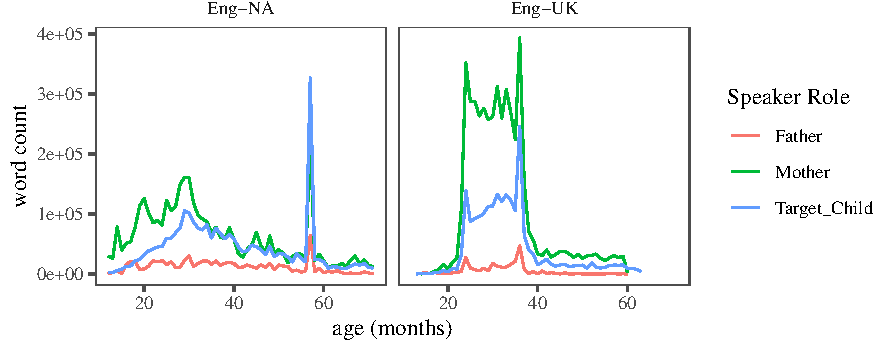
\includegraphics{figs/corpusDensityPlot-1} 

}

\caption{Frequency for all the words in the North America and UK corpora of CHILDES.}\label{fig:corpusDensityPlot}
\end{figure}

\hypertarget{properties-of-childes-corpora}{%
\subsection{Properties of CHILDES Corpora}\label{properties-of-childes-corpora}}

In this section, I report some results on the distribution of words and utterances among the speakers in our collection of corpora. The collection contained 14,159,609 words. Table (\ref{tab:countTable}) shows the total number of \emph{and}'s, \emph{or}'s, and words in the speech of children, fathers, and mothers. The collection contains 9 times more words for mothers compared to fathers and 2 more words for mothers compared to children. Therefore, the collection is more representative of the mother-child interactions than father-child interactions. Compared to \emph{or}, the word \emph{and} is 10.80 times more likely in the speech of mothers, 9.20 times more likely in the speech of fathers, and 30.30 times more likely in the speech of children. Overall, \emph{and} is 13.35 times more likely than \emph{or} in this collection which is close to the rate reported by Morris (2008) who used a smaller subset of CHILDES. He extracted 5,994 instances of \emph{and} and 465 instances of \emph{or} and found that overall, \emph{and} was 12.89 times more frequent than \emph{or} in parent-child interactions.

\begin{table}

\caption{\label{tab:countTable}Number of \textit{and}'s, \textit{or}'s, and the total number of words in the speech of children and their parents in English-North America and English-UK collections after exclusions.}
\centering
\begin{tabular}[t]{l|r|r|r}
\hline
Speaker Role & and & or & total\\
\hline
Father & 15,488 & 1,683 & 967,075\\
\hline
Mother & 153,781 & 14,288 & 8,511,478\\
\hline
Target\_Child & 78,443 & 2,590 & 4,681,056\\
\hline
\end{tabular}
\end{table}

Figure \ref{fig:wordsByAge} shows the number of words spoken by parents and children at each month of the child's development. The words in the collection are not distributed uniformly and there is a high concentration of data between the ages of 20 and 40 months (around 2 to 3 years of age). There is also a high concentration around 60 months (5 years of age). The speech of fathers shows a relatively low word-count across all ages. Therefore, in our analyses we should be more cautious in drawing conclusions about the speech of fathers generally, and the speech of mothers and children after age 5.
The distribution of function words is sensitive to the type of utterance or more broadly the type of speech act produced by speakers. Therefore, it is important to check the distribution of speech acts in corpora when studying different function words. Since it is hard to classify and quantify speech acts automatically, here I use utterance type as a proxy for speech acts. I investigate the distribution of declaratives, questions, and imperatives in this collection of corpora on parent-child interactions. Figure \ref{fig:totalUtteranceTypePlot} shows the distribution of different utterance types in the speech of parents and children. Overall, most utterances are either declaratives or questions, and there are more declaratives than questions in this collection. While mothers and fathers show similar proportions of declaratives and questions in their speech, children produce a lower proportion of questions and higher proportion of declaratives than their parents.

\begin{figure}[tb]

{\centering 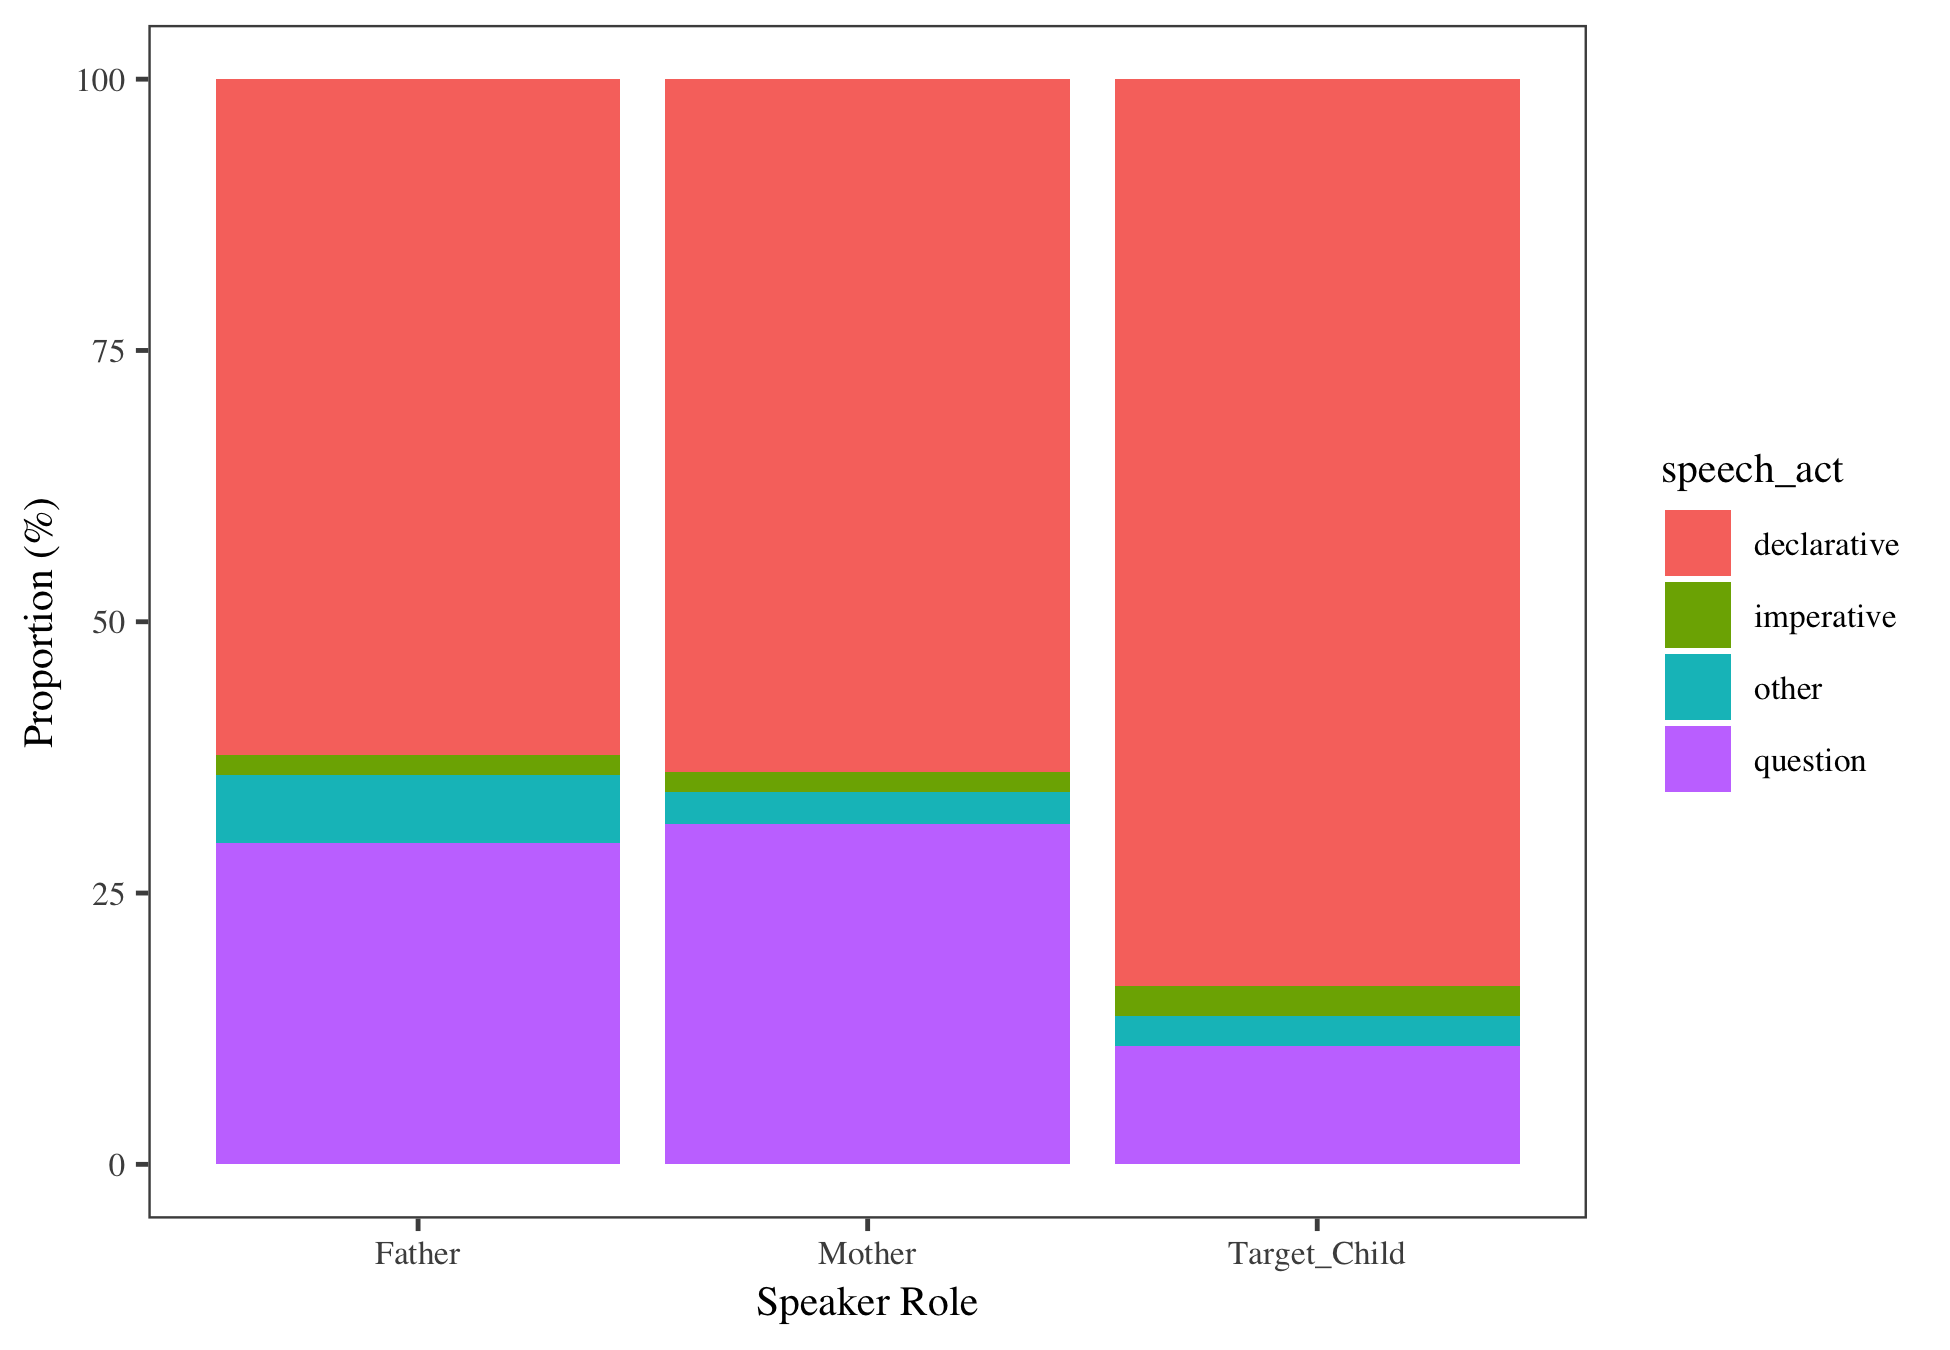
\includegraphics{figs/totalUtteranceTypePlot-1} 

}

\caption{The proportion of declaratives and questions in children's and parents' utterances.}\label{fig:totalUtteranceTypePlot}
\end{figure}

Figure \ref{fig:utteranceTypeByAgePlot} shows the developmental trend of declaratives and questions between the ages of one and six. Children start with only producing declaratives and add non-declarative utterances to their repertoire gradually until they get closer to the parents' rate around the age six. They also start with very few questions and increase the number of questions they ask gradually. It is important to note that the rates of declaratives and questions in children's speech do not reach the adult rate. These two figures show that parent-child interactions are asymmetric. Parents ask more questions and children produce more declaratives. This asymmetry also interacts with age: the speech of younger children has a higher proportion of declaratives than older children.

\begin{figure}
\centering
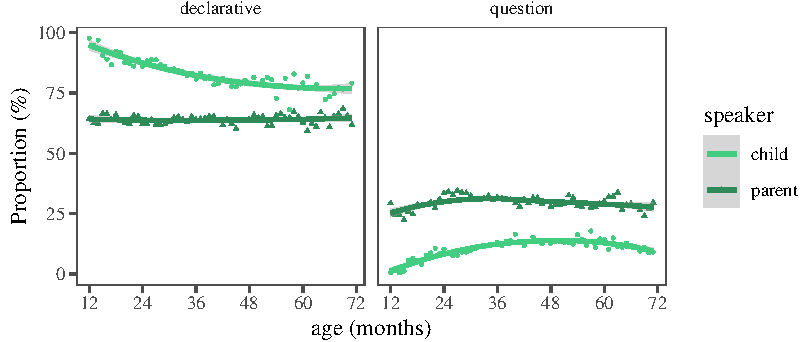
\includegraphics{figs/utteranceTypeByAgePlot-1.pdf}
\caption{\label{fig:utteranceTypeByAgePlot}Proportion of declaratives to questions in parent-child interactions by age.}
\end{figure}

The frequency of function words such as \emph{and} and \emph{or} may be affected by such conversational asymmetries if they are more likely to appear in some utterance types than others. Figure \ref{fig:CnctPropbySpeechAct} shows the proportion of \emph{and}'s and \emph{or}'s that appear in different utterance types in parents' and children's speech. In parents' speech, \emph{and} appears more often in declaratives (around 60\% in declaratives and 20\% in questions). On the other hand, \emph{or} appears more often in questions than declaratives, although this difference is small in mothers. In children's speech, both \emph{and} and \emph{or} appear most often in declaratives. However, children have a higher proportion of \emph{or} in questions than \emph{and} in questions.

The differences in the distribution of utterance types can affect our interpretation of the corpus data on function words such as \emph{and} and \emph{or} in three ways. First, since the collection contains more declaratives than questions, it may reflect the frequency and diversity of function words like \emph{and} that appear in declaratives better. Second, since children produce more declaratives and fewer questions than parents, we may underestimate children's knowledge of function words like \emph{or} that are frequent in questions. Third, given that the percentage of questions in the speech of children increases as they get older, function words like \emph{or} that are more likely to appear in questions may appear infrequent in the early stages and more frequent in the later stages of children's development. In other words, function words like \emph{or} that are common in questions may show a seeming delay in production which is possibly due to the development of questions in children's speech. Therefore, in studying children's productions of function words, it is important to look at their relative frequencies in different utterance types as well as the overall trends. This is the approach I pursue in the next section.

\begin{figure}[tb]

{\centering 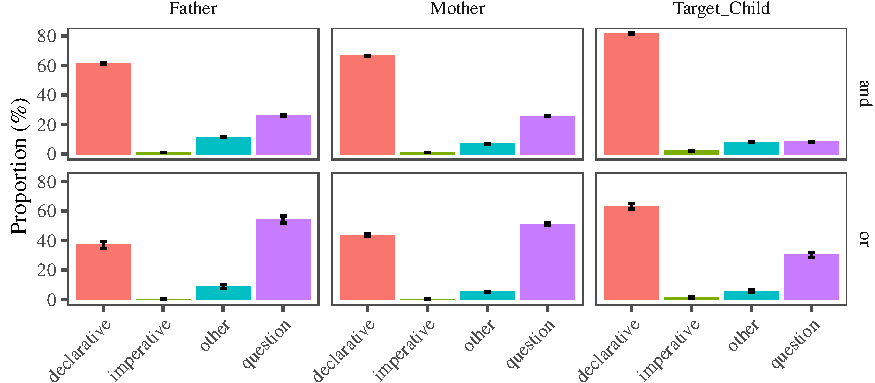
\includegraphics{figs/CnctPropbySpeechAct-1} 

}

\caption{The proportion of \textit{and} and \textit{or} in different utterance types in the speech of parents and children.}\label{fig:CnctPropbySpeechAct}
\end{figure}

=======
>>>>>>> master
\begin{longtable}[]{@{}ccc@{}}
\caption{\label{tab:providence} Information on the participants in the Providence Corpus. Ethan was diagnosed with Asperger's syndrome and therefore was excluded from this study.}\tabularnewline
\toprule
Name & Age Range & Sessions\tabularnewline
\midrule
\endfirsthead
\toprule
Name & Age Range & Sessions\tabularnewline
\midrule
\endhead
Alex & 1;04.28-3;05.16 & 51\tabularnewline
Ethan & 0;11.04-2;11.01 & 50\tabularnewline
Lily & 1;01.02-4;00.02 & 80\tabularnewline
Naima & 0;11.27-3;10.10 & 88\tabularnewline
Violet & 1;02.00-3;11.24 & 51\tabularnewline
William & 1;04.12-3;04.18 & 44\tabularnewline
\bottomrule
\end{longtable}

\hypertarget{annotation-categories-1}{%
\subsection{Annotation Categories}\label{annotation-categories-1}}

\begin{longtable}[]{@{}lll@{}}
\caption{\label{tab:connectiveInterpretaion} Annotation classes for connective interpretation}\tabularnewline
\toprule
\begin{minipage}[b]{0.06\columnwidth}\raggedright
Class\strut
\end{minipage} & \begin{minipage}[b]{0.36\columnwidth}\raggedright
Meaning\strut
\end{minipage} & \begin{minipage}[b]{0.49\columnwidth}\raggedright
Examples\strut
\end{minipage}\tabularnewline
\midrule
\endfirsthead
\toprule
\begin{minipage}[b]{0.06\columnwidth}\raggedright
Class\strut
\end{minipage} & \begin{minipage}[b]{0.36\columnwidth}\raggedright
Meaning\strut
\end{minipage} & \begin{minipage}[b]{0.49\columnwidth}\raggedright
Examples\strut
\end{minipage}\tabularnewline
\midrule
\endhead
\begin{minipage}[t]{0.06\columnwidth}\raggedright
AND\strut
\end{minipage} & \begin{minipage}[t]{0.36\columnwidth}\raggedright
Both propositions are true\strut
\end{minipage} & \begin{minipage}[t]{0.49\columnwidth}\raggedright
\emph{\enquote{I'm just gonna empty this and then I'll be out of the kitchen.} -- \enquote{I'll mix them together or I could mix it with carrot, too.}}\strut
\end{minipage}\tabularnewline
\begin{minipage}[t]{0.06\columnwidth}\raggedright
IOR\strut
\end{minipage} & \begin{minipage}[t]{0.36\columnwidth}\raggedright
One or both propositions are true\strut
\end{minipage} & \begin{minipage}[t]{0.49\columnwidth}\raggedright
\emph{\enquote{You should use a spoon or a fork.} -- \enquote{Ask a grownup for some juice or water or soy milk.}}\strut
\end{minipage}\tabularnewline
\begin{minipage}[t]{0.06\columnwidth}\raggedright
XOR\strut
\end{minipage} & \begin{minipage}[t]{0.36\columnwidth}\raggedright
Only one proposition is true\strut
\end{minipage} & \begin{minipage}[t]{0.49\columnwidth}\raggedright
\emph{\enquote{Is that a hyena? or a leopard?} -- \enquote{We're gonna do things one way or the other.}}\strut
\end{minipage}\tabularnewline
\begin{minipage}[t]{0.06\columnwidth}\raggedright
NOR\strut
\end{minipage} & \begin{minipage}[t]{0.36\columnwidth}\raggedright
Neither proposition is true\strut
\end{minipage} & \begin{minipage}[t]{0.49\columnwidth}\raggedright
\emph{\enquote{I wouldn't say boo to one goose or three.} -- \enquote{She found she lacked talent for hiding in trees, for chirping like crickets, or humming like bees.}}\strut
\end{minipage}\tabularnewline
\begin{minipage}[t]{0.06\columnwidth}\raggedright
IFF\strut
\end{minipage} & \begin{minipage}[t]{0.36\columnwidth}\raggedright
Either both propositions are true or both are false\strut
\end{minipage} & \begin{minipage}[t]{0.49\columnwidth}\raggedright
\emph{\enquote{Put them {[}crayons{]} up here and you can get down. -- Come over here and I'll show you.}}\strut
\end{minipage}\tabularnewline
\begin{minipage}[t]{0.06\columnwidth}\raggedright
NAB\strut
\end{minipage} & \begin{minipage}[t]{0.36\columnwidth}\raggedright
The first proposition is false, the second is true.\strut
\end{minipage} & \begin{minipage}[t]{0.49\columnwidth}\raggedright
\emph{\enquote{There's an Oatio here, or actually, there's a wheat here.}}\strut
\end{minipage}\tabularnewline
\bottomrule
\end{longtable}

\begin{longtable}[]{@{}lll@{}}
\caption{\label{tab:intonationTypes} Definitions of the intonation types and their examples.}\tabularnewline
\toprule
\begin{minipage}[b]{0.11\columnwidth}\raggedright
Intonation\strut
\end{minipage} & \begin{minipage}[b]{0.46\columnwidth}\raggedright
Definitions\strut
\end{minipage} & \begin{minipage}[b]{0.35\columnwidth}\raggedright
Examples\strut
\end{minipage}\tabularnewline
\midrule
\endfirsthead
\toprule
\begin{minipage}[b]{0.11\columnwidth}\raggedright
Intonation\strut
\end{minipage} & \begin{minipage}[b]{0.46\columnwidth}\raggedright
Definitions\strut
\end{minipage} & \begin{minipage}[b]{0.35\columnwidth}\raggedright
Examples\strut
\end{minipage}\tabularnewline
\midrule
\endhead
\begin{minipage}[t]{0.11\columnwidth}\raggedright
Flat\strut
\end{minipage} & \begin{minipage}[t]{0.46\columnwidth}\raggedright
Intonation does not show any substantial rise at the end of the sentence.\strut
\end{minipage} & \begin{minipage}[t]{0.35\columnwidth}\raggedright
\emph{\enquote{I don't hear any meows or bow-wow-wows.}}\strut
\end{minipage}\tabularnewline
\begin{minipage}[t]{0.11\columnwidth}\raggedright
Rise\strut
\end{minipage} & \begin{minipage}[t]{0.46\columnwidth}\raggedright
There is a substantial intonation rise on each disjunct or generally on both.\strut
\end{minipage} & \begin{minipage}[t]{0.35\columnwidth}\raggedright
\emph{\enquote{Do you want some seaweed? or some wheat germ?}}\strut
\end{minipage}\tabularnewline
\begin{minipage}[t]{0.11\columnwidth}\raggedright
Rise-Fall\strut
\end{minipage} & \begin{minipage}[t]{0.46\columnwidth}\raggedright
There is a substantial rise on the non-final disjunct(s), and a fall on the final disjunct.\strut
\end{minipage} & \begin{minipage}[t]{0.35\columnwidth}\raggedright
\emph{\enquote{Is that big Q or little q?} -- \enquote{(are) You patting them, petting them, or slapping them?}}\strut
\end{minipage}\tabularnewline
\bottomrule
\end{longtable}

\begin{longtable}[]{@{}lll@{}}
\caption{\label{tab:utteranceTypes} Definitions of the utterance types and their examples.}\tabularnewline
\toprule
\begin{minipage}[b]{0.18\columnwidth}\raggedright
Utterance Types\strut
\end{minipage} & \begin{minipage}[b]{0.42\columnwidth}\raggedright
Definitions\strut
\end{minipage} & \begin{minipage}[b]{0.32\columnwidth}\raggedright
Examples\strut
\end{minipage}\tabularnewline
\midrule
\endfirsthead
\toprule
\begin{minipage}[b]{0.18\columnwidth}\raggedright
Utterance Types\strut
\end{minipage} & \begin{minipage}[b]{0.42\columnwidth}\raggedright
Definitions\strut
\end{minipage} & \begin{minipage}[b]{0.32\columnwidth}\raggedright
Examples\strut
\end{minipage}\tabularnewline
\midrule
\endhead
\begin{minipage}[t]{0.18\columnwidth}\raggedright
Declarative\strut
\end{minipage} & \begin{minipage}[t]{0.42\columnwidth}\raggedright
A statement with a subject-verb-object word order and a flat intonation.\strut
\end{minipage} & \begin{minipage}[t]{0.32\columnwidth}\raggedright
\emph{\enquote{It looks a little bit like a drum stick or a mallet.}}\strut
\end{minipage}\tabularnewline
\begin{minipage}[t]{0.18\columnwidth}\raggedright
Interrogative\strut
\end{minipage} & \begin{minipage}[t]{0.42\columnwidth}\raggedright
A question with either subject-auxiliary inversion or a rising terminal intonation.\strut
\end{minipage} & \begin{minipage}[t]{0.32\columnwidth}\raggedright
\emph{\enquote{Is that a dog or a cat?}}\strut
\end{minipage}\tabularnewline
\begin{minipage}[t]{0.18\columnwidth}\raggedright
Imperative\strut
\end{minipage} & \begin{minipage}[t]{0.42\columnwidth}\raggedright
A directive with an uninflected verb and no subject\strut
\end{minipage} & \begin{minipage}[t]{0.32\columnwidth}\raggedright
\emph{\enquote{Have a little more French toast or have some of your juice.}}\strut
\end{minipage}\tabularnewline
\bottomrule
\end{longtable}

\begin{longtable}[]{@{}lll@{}}
\caption{\label{tab:syntacticLevel} Definitions of the syntactic levels and their examples.}\tabularnewline
\toprule
\begin{minipage}[b]{0.17\columnwidth}\raggedright
Syntactic Level\strut
\end{minipage} & \begin{minipage}[b]{0.37\columnwidth}\raggedright
Definitions\strut
\end{minipage} & \begin{minipage}[b]{0.37\columnwidth}\raggedright
Examples\strut
\end{minipage}\tabularnewline
\midrule
\endfirsthead
\toprule
\begin{minipage}[b]{0.17\columnwidth}\raggedright
Syntactic Level\strut
\end{minipage} & \begin{minipage}[b]{0.37\columnwidth}\raggedright
Definitions\strut
\end{minipage} & \begin{minipage}[b]{0.37\columnwidth}\raggedright
Examples\strut
\end{minipage}\tabularnewline
\midrule
\endhead
\begin{minipage}[t]{0.17\columnwidth}\raggedright
Clausal\strut
\end{minipage} & \begin{minipage}[t]{0.37\columnwidth}\raggedright
The coordinands are sentences, clauses, verb phrases, or verbs.\strut
\end{minipage} & \begin{minipage}[t]{0.37\columnwidth}\raggedright
\emph{\enquote{Does he lose his tail sometimes and Pooh helps him and puts it back on?}}\strut
\end{minipage}\tabularnewline
\begin{minipage}[t]{0.17\columnwidth}\raggedright
Sub-clausal\strut
\end{minipage} & \begin{minipage}[t]{0.37\columnwidth}\raggedright
The coordinands are nouns, adjectives, noun phrases, determiner phrases, or prepositional phrases.\strut
\end{minipage} & \begin{minipage}[t]{0.37\columnwidth}\raggedright
\emph{\enquote{Hollies can be bushes or trees.}}\strut
\end{minipage}\tabularnewline
\bottomrule
\end{longtable}

\begin{longtable}[]{@{}lll@{}}
\caption{\label{tab:consistencyType} Definitions of consistency types and their examples.}\tabularnewline
\toprule
\begin{minipage}[b]{0.15\columnwidth}\raggedright
Consistency\strut
\end{minipage} & \begin{minipage}[b]{0.28\columnwidth}\raggedright
Definitions\strut
\end{minipage} & \begin{minipage}[b]{0.48\columnwidth}\raggedright
Examples\strut
\end{minipage}\tabularnewline
\midrule
\endfirsthead
\toprule
\begin{minipage}[b]{0.15\columnwidth}\raggedright
Consistency\strut
\end{minipage} & \begin{minipage}[b]{0.28\columnwidth}\raggedright
Definitions\strut
\end{minipage} & \begin{minipage}[b]{0.48\columnwidth}\raggedright
Examples\strut
\end{minipage}\tabularnewline
\midrule
\endhead
\begin{minipage}[t]{0.15\columnwidth}\raggedright
Consistent\strut
\end{minipage} & \begin{minipage}[t]{0.28\columnwidth}\raggedright
The coordinands can be true at the same time.\strut
\end{minipage} & \begin{minipage}[t]{0.48\columnwidth}\raggedright
\emph{\enquote{We could spell some things with a pen or draw some pictures.}}\strut
\end{minipage}\tabularnewline
\begin{minipage}[t]{0.15\columnwidth}\raggedright
Inconsistent\strut
\end{minipage} & \begin{minipage}[t]{0.28\columnwidth}\raggedright
The coordinands cannot be true at the same time.\strut
\end{minipage} & \begin{minipage}[t]{0.48\columnwidth}\raggedright
\emph{\enquote{Do you want to stay or go?}}\strut
\end{minipage}\tabularnewline
\bottomrule
\end{longtable}

\begin{longtable}[]{@{}lll@{}}
\caption{\label{tab:speechActs} Definitions of the communicative functions and their examples.}\tabularnewline
\toprule
\begin{minipage}[b]{0.13\columnwidth}\raggedright
Function\strut
\end{minipage} & \begin{minipage}[b]{0.45\columnwidth}\raggedright
Definitions\strut
\end{minipage} & \begin{minipage}[b]{0.33\columnwidth}\raggedright
Examples\strut
\end{minipage}\tabularnewline
\midrule
\endfirsthead
\toprule
\begin{minipage}[b]{0.13\columnwidth}\raggedright
Function\strut
\end{minipage} & \begin{minipage}[b]{0.45\columnwidth}\raggedright
Definitions\strut
\end{minipage} & \begin{minipage}[b]{0.33\columnwidth}\raggedright
Examples\strut
\end{minipage}\tabularnewline
\midrule
\endhead
\begin{minipage}[t]{0.13\columnwidth}\raggedright
Descriptions\strut
\end{minipage} & \begin{minipage}[t]{0.45\columnwidth}\raggedright
Describing what the world is like or asking about it. The primary goal is to inform the addressee about how things are.\strut
\end{minipage} & \begin{minipage}[t]{0.33\columnwidth}\raggedright
\enquote{\emph{It's not in the ditch or the drain pipe.}}\strut
\end{minipage}\tabularnewline
\begin{minipage}[t]{0.13\columnwidth}\raggedright
Identifications\strut
\end{minipage} & \begin{minipage}[t]{0.45\columnwidth}\raggedright
Identifying the category membership or an attribute of an object. Speaker has uncertainty. A subtype of \enquote{Description}.\strut
\end{minipage} & \begin{minipage}[t]{0.33\columnwidth}\raggedright
\enquote{\emph{Is that a ball or a balloon honey?}}\strut
\end{minipage}\tabularnewline
\begin{minipage}[t]{0.13\columnwidth}\raggedright
Definitions and Examples\strut
\end{minipage} & \begin{minipage}[t]{0.45\columnwidth}\raggedright
Providing labels for a category or examples for it. Speaker is certain. Subtype of Description.\strut
\end{minipage} & \begin{minipage}[t]{0.33\columnwidth}\raggedright
\emph{\enquote{This is a cup or a mug.} -- \enquote{berries like blueberry or raspberry}}\strut
\end{minipage}\tabularnewline
\begin{minipage}[t]{0.13\columnwidth}\raggedright
Preferences\strut
\end{minipage} & \begin{minipage}[t]{0.45\columnwidth}\raggedright
Asking what the addressee wants or would like or stating what the speaker wants or would like\strut
\end{minipage} & \begin{minipage}[t]{0.33\columnwidth}\raggedright
\emph{\enquote{Do you wanna play pizza or read the book?}}\strut
\end{minipage}\tabularnewline
\begin{minipage}[t]{0.13\columnwidth}\raggedright
Options\strut
\end{minipage} & \begin{minipage}[t]{0.45\columnwidth}\raggedright
Either asking or listing what one can or is allowed to do. Giving permission, asking for permission, or describing the possibilities. Often the modal \enquote{can} is either present or can be inserted.\strut
\end{minipage} & \begin{minipage}[t]{0.33\columnwidth}\raggedright
\emph{\enquote{You could have wheat or rice.}}\strut
\end{minipage}\tabularnewline
\begin{minipage}[t]{0.13\columnwidth}\raggedright
Directives\strut
\end{minipage} & \begin{minipage}[t]{0.45\columnwidth}\raggedright
Directing the addressee to act or not act in a particular way. Common patterns include \enquote{let's do \ldots{}}, \enquote{Why don't you do \ldots{}}, or prohibitions such as \enquote{Don't \ldots{}}. The difference with \enquote{options} is that the speaker expects the directive to be carried out by the addressee. There is no such expectation for \enquote{options}.\strut
\end{minipage} & \begin{minipage}[t]{0.33\columnwidth}\raggedright
\emph{\enquote{let's go back and play with your ball or we'll read your book.}}\strut
\end{minipage}\tabularnewline
\begin{minipage}[t]{0.13\columnwidth}\raggedright
Clarifications\strut
\end{minipage} & \begin{minipage}[t]{0.45\columnwidth}\raggedright
Something is said or done as a communicative act but the speaker has uncertainty with respect to the form or the content.\strut
\end{minipage} & \begin{minipage}[t]{0.33\columnwidth}\raggedright
\emph{\enquote{You mean boba or bubble?}}\strut
\end{minipage}\tabularnewline
\begin{minipage}[t]{0.13\columnwidth}\raggedright
Repairs\strut
\end{minipage} & \begin{minipage}[t]{0.45\columnwidth}\raggedright
Speaker correcting herself on something she said (self repair) or correcting the addressee (other repair). The second disjunct is what holds and is intended by the speaker. The speaker does not have uncertainty with respect to what actually holds.\strut
\end{minipage} & \begin{minipage}[t]{0.33\columnwidth}\raggedright
\emph{\enquote{There's an Oatio here, or actually, there's a wheat here.}}\strut
\end{minipage}\tabularnewline
\begin{minipage}[t]{0.13\columnwidth}\raggedright
Conditionals\strut
\end{minipage} & \begin{minipage}[t]{0.45\columnwidth}\raggedright
Explaining in the second coordinand, what would follow if the first coordinand is (or is not) followed. Subtype of Directive.\strut
\end{minipage} & \begin{minipage}[t]{0.33\columnwidth}\raggedright
\emph{\enquote{Put that out of your mouth, or I'm gonna put it away.}} -- \emph{\enquote{Come over here and I'll show you.}}\strut
\end{minipage}\tabularnewline
\begin{minipage}[t]{0.13\columnwidth}\raggedright
Unconditionals\strut
\end{minipage} & \begin{minipage}[t]{0.45\columnwidth}\raggedright
Denying the dependence of something on a set of conditions. Typical format: \enquote{Whether X or Y, Z}. Subtype of Descriptions.\strut
\end{minipage} & \begin{minipage}[t]{0.33\columnwidth}\raggedright
\emph{\enquote{Ready or not, here I come!}} (playing hide and seek)\strut
\end{minipage}\tabularnewline
\bottomrule
\end{longtable}

\begin{longtable}[]{@{}lll@{}}
\caption{\label{tab:answerTypes} Definitions of answer types and their examples.}\tabularnewline
\toprule
\begin{minipage}[b]{0.17\columnwidth}\raggedright
Type\strut
\end{minipage} & \begin{minipage}[b]{0.42\columnwidth}\raggedright
Definitions\strut
\end{minipage} & \begin{minipage}[b]{0.33\columnwidth}\raggedright
Examples\strut
\end{minipage}\tabularnewline
\midrule
\endfirsthead
\toprule
\begin{minipage}[b]{0.17\columnwidth}\raggedright
Type\strut
\end{minipage} & \begin{minipage}[b]{0.42\columnwidth}\raggedright
Definitions\strut
\end{minipage} & \begin{minipage}[b]{0.33\columnwidth}\raggedright
Examples\strut
\end{minipage}\tabularnewline
\midrule
\endhead
\begin{minipage}[t]{0.17\columnwidth}\raggedright
No Answer\strut
\end{minipage} & \begin{minipage}[t]{0.42\columnwidth}\raggedright
The child provides no answer to the question.\strut
\end{minipage} & \begin{minipage}[t]{0.33\columnwidth}\raggedright
Mother: \emph{\enquote{Would you like to eat some applesauce or some carrots?}} Child: \emph{\enquote{Guess what Max!}}\strut
\end{minipage}\tabularnewline
\begin{minipage}[t]{0.17\columnwidth}\raggedright
YN\strut
\end{minipage} & \begin{minipage}[t]{0.42\columnwidth}\raggedright
The child responds with \emph{yes} or \emph{no}.\strut
\end{minipage} & \begin{minipage}[t]{0.33\columnwidth}\raggedright
Father: \emph{\enquote{Can I finish eating one or two more bites of my cereal?}} Child: \emph{\enquote{No.}}\strut
\end{minipage}\tabularnewline
\begin{minipage}[t]{0.17\columnwidth}\raggedright
AB\strut
\end{minipage} & \begin{minipage}[t]{0.42\columnwidth}\raggedright
The child responds with one of the disjuncts (alternatives).\strut
\end{minipage} & \begin{minipage}[t]{0.33\columnwidth}\raggedright
Mother: \emph{\enquote{Is she a baby elephant or is she a toddler elephant?}} Child: \emph{\enquote{It's a baby. She has a tail.}}\strut
\end{minipage}\tabularnewline
\bottomrule
\end{longtable}

\hypertarget{inter-annotator-agreement}{%
\subsection{Inter-annotator agreement}\label{inter-annotator-agreement}}

Figure \ref{fig:oReliabilityPlot} shows the percentage agreement and the kappa values for each annotation category over the 8 iterations.

\begin{figure}[tb]

{\centering 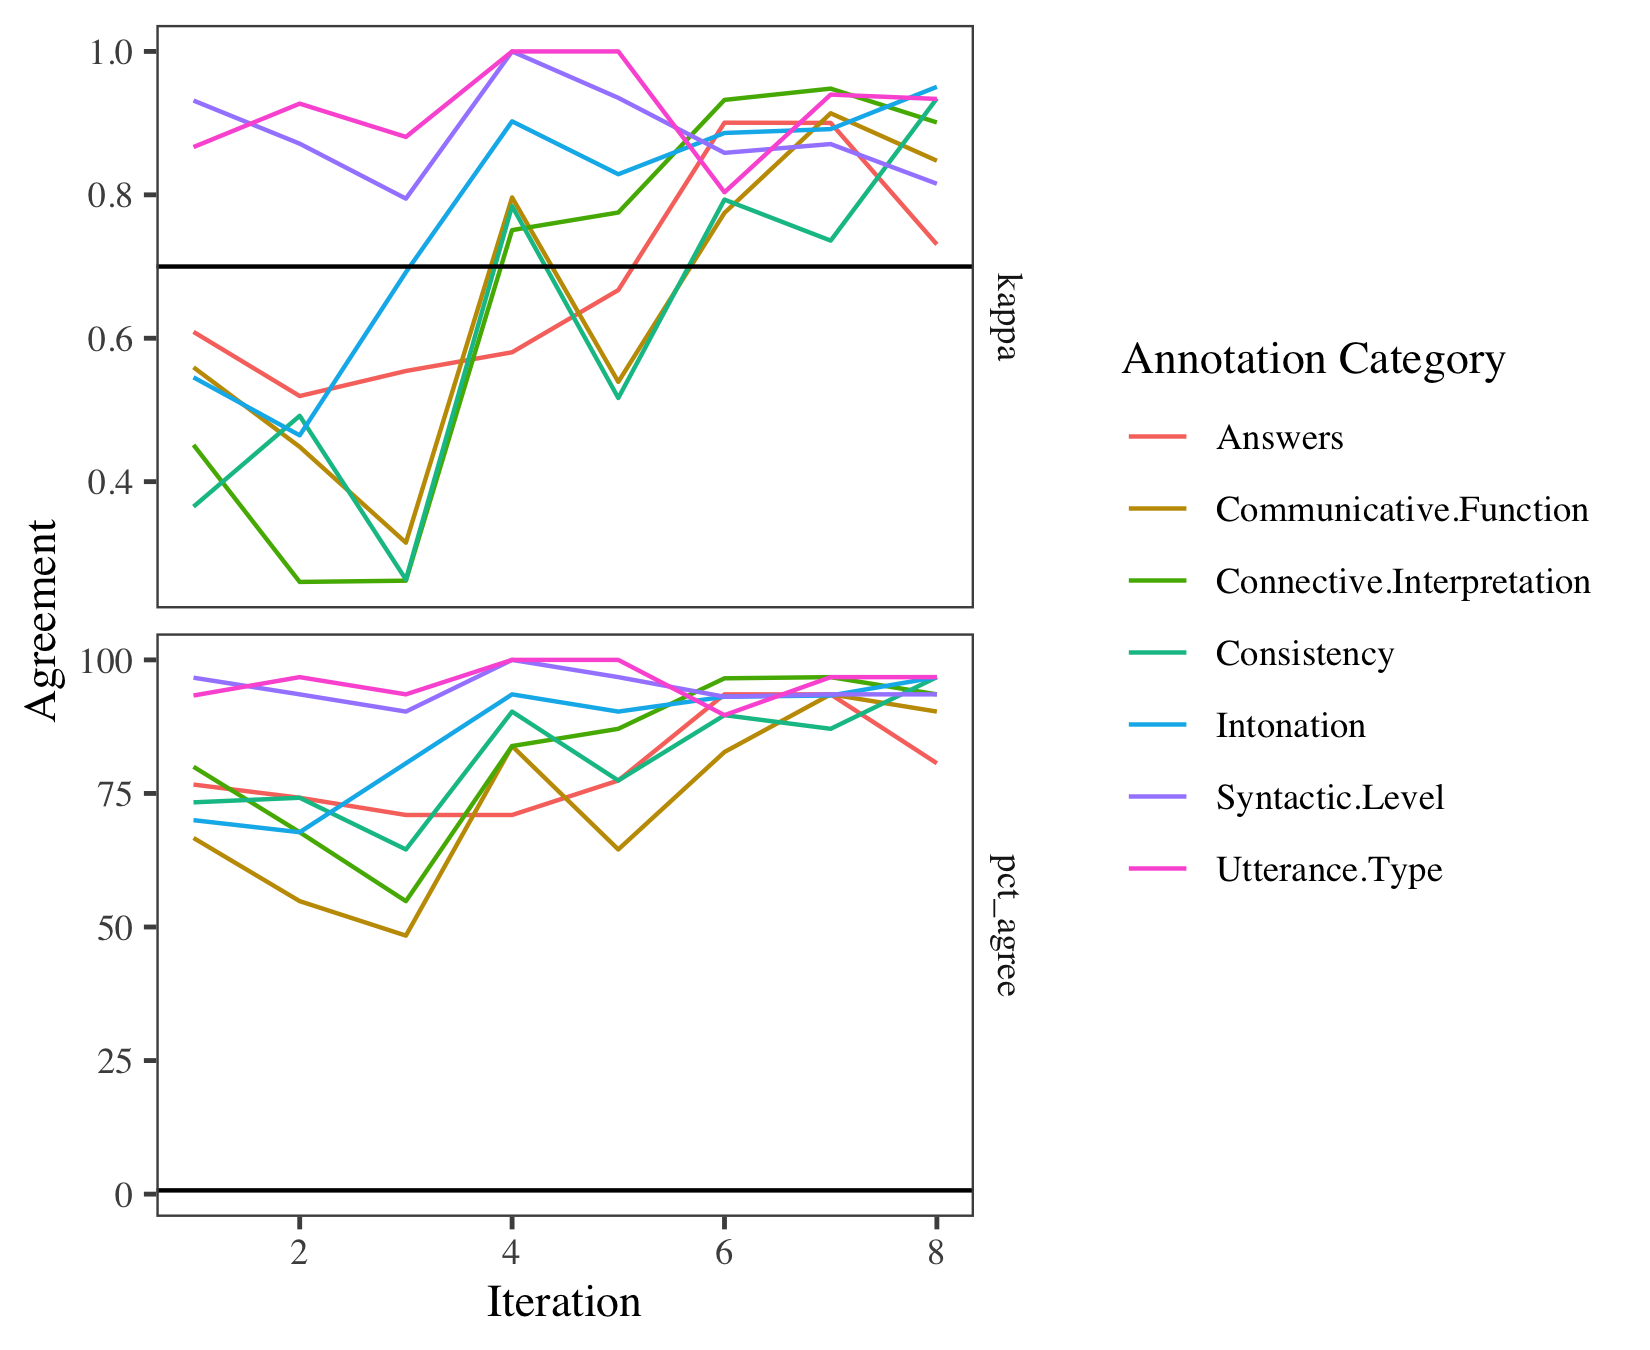
\includegraphics{figs/oReliabilityPlot-1} 

}

\caption{Inter-annotator agreement for disjunction examples.}\label{fig:oReliabilityPlot}
\end{figure}

Agreement in the following three categories showed substantial improvement after better and more precise definitions and annotation criteria were developed: connective interpretation, intonation, and communicative function. First, connective interpretation showed major improvements after annotators developed more precise criteria for selecting the propositions under discussion and separately wrote down the two propositions connected by the connective word. For example, if the original utterance was \enquote{do you want milk or juice?}, the annotators wrote \enquote{you want milk, you want juice} as the two propositions under discussion. This exercise clarified the exact propositions under discussion and sharpened annotator intuitions with respect to the connective interpretation that is communicated by the utterance. Second, annotators improved agreement on intonation by reconstructing an utterance's intonation for all three intonation categories. For example, the annotator would examine the same sentence \enquote{do you want coffee or tea?} with a rise-fall, a rise, and a flat intonation. Then the annotator would listen to the actual utterance and see which one most resembled the actual utterance. This method helped annotators judge the intonation of an utterance more accurately. Finally, agreement on communicative functions improved as the definitions were made more precise. For example, the definition of \enquote{directives} in Table \ref{tab:speechActs} explicitly mentions the difference between \enquote{directives} and \enquote{options}. Clarifying the definitions of communicative functions helped improve annotator agreement.

Inter-annotator reliability for conjunction was calculated in the same way. Two different annotators coded 300 utterances of \emph{and}. Inter-annotator reliability was calculated over 10 iterations of 30 examples. Figure \ref{fig:andReliabilityPlot} shows the percentage agreement between the annotators as well as the kappa values for each iteration. Despite high percentage agreement between annotators, the kappa values did not pass the set threshold of 0.7 in three consecutive iterations. This paradoxical result is mainly due to a property of kappa. An imbalance in the prevalence of annotation categories can drastically lower its value. When one category is extremely common with high agreement while other categories are rare, kappa will be low (Cicchetti \& Feinstein, 1990; Feinstein \& Cicchetti, 1990). In almost all annotated categories for conjunction, there was one class that was extremely prevalent. In such cases, it is more informative to look at the class specific agreement for the prevalent category than the overall agreement measured by Kappa (Cicchetti \& Feinstein, 1990; Feinstein \& Cicchetti, 1990).

\begin{figure}[tb]

{\centering 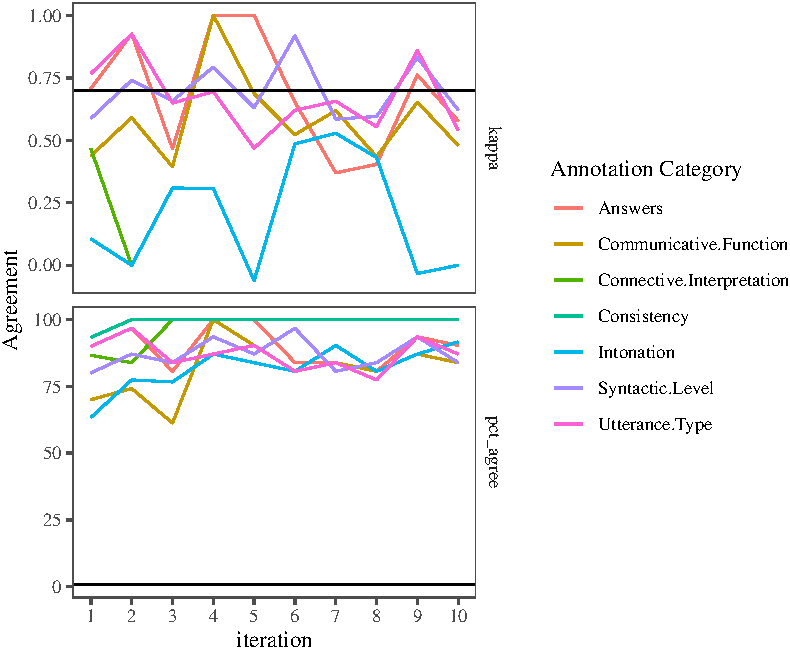
\includegraphics{figs/andReliabilityPlot-1} 

}

\caption{Inter-annotator agreement for conjunction examples.}\label{fig:andReliabilityPlot}
\end{figure}

Table \ref{tab:andAgreeStats} lists the dominant classes as well as their prevalence, the values of class specific agreement index, and category agreement index (Kappa). Class specific agreement index is defined as \(2n_{ii}/n_{i.}+n_{.i}\), where \(i\) represents the class's row/column number in the category's confusion matrix, \(n\) the number of annotations in a cell, and the dot ranges over all the row/column numbers (Fleiss, Levin, \& Paik, 2013, p. 600; Ubersax, 2009). The class specific agreement indices are high for all the most prevalent classes showing that the annotators had very high agreement on these class, even though the general agreement index (Kappa) was often low. The most extreme case is the category \enquote{consistency} where almost all instances were annotated as \enquote{consistent} with perfect class specific agreement but low overall Kappa. In the case of utterance type and syntactic level where the distribution of instances across classes was more even, the general index of agreement Kappa is also high. In general, examples of conjunction showed little variability across annotation categories and mostly fell into one class within each category. Annotators had high agreement for these dominant classes.

\begin{table}

\caption{\label{tab:andAgreeStats}Most prevalent annotation class in each annotation category with the values of class agreement indeces and category agreement indeces (Kappa).}
\centering
\begin{tabular}[t]{l|l|r|r|r}
\hline
Annotation Category & Class & Prevalence & Class Agreement Index & Kappa\\
\hline
intonation & flat & 0.86 & 0.89 & 0.24\\
\hline
interpretation & AND & 0.96 & 0.98 & 0.39\\
\hline
answer & NA & 0.84 & 0.94 & 0.67\\
\hline
utterance\_type & declarative & 0.76 & 0.94 & 0.70\\
\hline
communicative\_function & description & 0.77 & 0.90 & 0.59\\
\hline
syntactic\_level & clausal & 0.67 & 0.91 & 0.70\\
\hline
consistency & consistent & 0.99 & 1.00 & 0.50\\
\hline
\end{tabular}
\end{table}

\setlength{\parindent}{-0.5in}
\setlength{\leftskip}{0.5in}

\hypertarget{refs}{}
\leavevmode\hypertarget{ref-baldwin1993infants}{}%
Baldwin, D. (1993). Infants' ability to consult the speaker for clues to word reference. \emph{Journal of Child Language}, \emph{20}(2), 395--418.

\leavevmode\hypertarget{ref-braine1981development}{}%
Braine, M. D., \& Rumain, B. (1981). Development of comprehension of ``or'': Evidence for a sequence of competencies. \emph{Journal of Experimental Child Psychology}, \emph{31}(1), 46--70.

\leavevmode\hypertarget{ref-breiman2001random}{}%
Breiman, L. (2001). Random forests. \emph{Machine Learning}, \emph{45}(1), 5--32.

\leavevmode\hypertarget{ref-breiman2017classification}{}%
Breiman, L. (2017). \emph{Classification and regression trees}. London: Routledge.

\leavevmode\hypertarget{ref-brown1957linguistic}{}%
Brown, R. W. (1957). Linguistic determinism and the part of speech. \emph{The Journal of Abnormal and Social Psychology}, \emph{55}(1), 1.

\leavevmode\hypertarget{ref-chierchia2001acquisition}{}%
Chierchia, G., Crain, S., Guasti, M. T., Gualmini, A., \& Meroni, L. (2001). The acquisition of disjunction: Evidence for a grammatical view of scalar implicatures. In \emph{Proceedings of the 25th Boston University conference on language development} (pp. 157--168). Somerville, MA: Cascadilla Press.

\leavevmode\hypertarget{ref-chierchia2004semantic}{}%
Chierchia, G., Guasti, M. T., Gualmini, A., Meroni, L., Crain, S., \& Foppolo, F. (2004). Semantic and pragmatic competence in children's and adults' comprehension of or. In I. Noveck \& D. Sperber (Eds.), \emph{Experimental pragmatics} (pp. 283--300). Basingstoke: Palgrave Macmillan.

\leavevmode\hypertarget{ref-cicchetti1990high}{}%
Cicchetti, D. V., \& Feinstein, A. R. (1990). High agreement but low kappa: II. Resolving the paradoxes. \emph{Journal of Clinical Epidemiology}, \emph{43}(6), 551--558.

\leavevmode\hypertarget{ref-clark1993lexicon}{}%
Clark, E. V. (1993). \emph{The lexicon in acquisition}. Cambridge University Press.

\leavevmode\hypertarget{ref-clark2009first}{}%
Clark, E. V. (2009). \emph{First language acquisition} (2nd ed.). Cambridge: Cambridge University Press.

\leavevmode\hypertarget{ref-crain2012emergence}{}%
Crain, S. (2012). \emph{The emergence of meaning}. Cambridge: Cambridge University Press.

\leavevmode\hypertarget{ref-crain2000acquisition}{}%
Crain, S., Gualmini, A., \& Meroni, L. (2000). The acquisition of logical words. \emph{LOGOS and Language}, \emph{1}, 49--59.

\leavevmode\hypertarget{ref-crain2008logic}{}%
Crain, S., \& Khlentzos, D. (2008). Is logic innate? \emph{Biolinguistics}, \emph{2}(1), 024--056.

\leavevmode\hypertarget{ref-crain2010logic}{}%
Crain, S., \& Khlentzos, D. (2010). The logic instinct. \emph{Mind \& Language}, \emph{25}(1), 30--65.

\leavevmode\hypertarget{ref-demuth2006word}{}%
Demuth, K., Culbertson, J., \& Alter, J. (2006). Word-minimality, epenthesis and coda licensing in the early acquisition of English. \emph{Language and Speech}, \emph{49}(2), 137--173.

\leavevmode\hypertarget{ref-feinstein1990high}{}%
Feinstein, A. R., \& Cicchetti, D. V. (1990). High agreement but low kappa: I. The problems of two paradoxes. \emph{Journal of Clinical Epidemiology}, \emph{43}(6), 543--549.

\leavevmode\hypertarget{ref-fleiss2013statistical}{}%
Fleiss, J. L., Levin, B., \& Paik, M. C. (2013). \emph{Statistical methods for rates and proportions}. New York: John Wiley \&amp; Sons.

\leavevmode\hypertarget{ref-geurts2006exclusive}{}%
Geurts, B. (2006). Exclusive disjunction without implicatures. \emph{Ms., University of Nijmegen}.

\leavevmode\hypertarget{ref-gini1912variabilita}{}%
Gini, C. (1912). Variabilità e mutabilità. \emph{Reprinted in Memorie Di Metodologica Statistica (Ed. Pizetti E, Salvemini, T). Rome: Libreria Eredi Virgilio Veschi}.

\leavevmode\hypertarget{ref-gleitman1990structural}{}%
Gleitman, L. (1990). The structural sources of verb meanings. \emph{Language Acquisition}, \emph{1}(1), 3--55.

\leavevmode\hypertarget{ref-goodman2008does}{}%
Goodman, J. C., Dale, P. S., \& Li, P. (2008). Does frequency count? Parental input and the acquisition of vocabulary. \emph{Journal of Child Language}, \emph{35}(3), 515--531.

\leavevmode\hypertarget{ref-grice1989studies}{}%
Grice, H. P. (1989). \emph{Studies in the way of words}. Cambridge, MA: Harvard University Press.

\leavevmode\hypertarget{ref-gualminicrain2002}{}%
Gualmini, A., \& Crain, S. (2002). Why no child or adult must learn de Morgan's laws. In \emph{Proceedings of the Boston University conference on language development}. Somerville, MA: Cascadilla Press.

\leavevmode\hypertarget{ref-gualmini2000}{}%
Gualmini, A., Crain, S., \& Meroni, L. (2000). Acqisition of disjunction in conditional sentences. In \emph{Proceedings of the boston university conference on language development}.

\leavevmode\hypertarget{ref-haspelmath2007}{}%
Haspelmath, M. (2007). Coordination. In T. Shopen (Ed.), \emph{Language typology and linguistic description,} Cambridge: Cambridge University Press.

\leavevmode\hypertarget{ref-ho1995random}{}%
Ho, T. K. (1995). Random decision forests. In \emph{Proceedings of the third international conference on document analysis and recognition} (Vol. 1, pp. 278--282). Washington, DC, USA: IEEE Computer Society.

\leavevmode\hypertarget{ref-hollich2000breaking}{}%
Hollich, G. J., Hirsh-Pasek, K., Golinkoff, R. M., Brand, R., Brown, E., Chung, H. L., \ldots{} Rocroi, C. (2000). Breaking the language barrier: An emergentist coalition model for the origins of word learning. \emph{Monographs of the Society for Research in Child Development}, \emph{65}(3), 1--123.

\leavevmode\hypertarget{ref-johansson1975preschool}{}%
Johansson, B. S., \& Sjolin, B. (1975). Preschool children's understanding of the coordinators ``and'' and ``or''. \emph{Journal of Experimental Child Psychology}, \emph{19}(2), 233--240.

\leavevmode\hypertarget{ref-kamp1973free}{}%
Kamp, H. (1973). Free choice permission. In \emph{Proceedings of the Aristotelian society} (Vol. 74, pp. 57--74).

\leavevmode\hypertarget{ref-levy1994words}{}%
Levy, E., \& Nelson, K. (1994). Words in discourse: A dialectical approach to the acquisition of meaning and use. \emph{Journal of Child Language}, \emph{21}(02), 367--389.

\leavevmode\hypertarget{ref-macwhinney2000childes}{}%
MacWhinney, B. (2000). \emph{The CHILDES project: The database} (Vol. 2). Mahwah, NJ: Erlbaum.

\leavevmode\hypertarget{ref-markman1990constraints}{}%
Markman, E. M. (1990). Constraints children place on word meanings. \emph{Cognitive Science}, \emph{14}(1), 57--77.

\leavevmode\hypertarget{ref-markman1984children}{}%
Markman, E. M., \& Hutchinson, J. E. (1984). Children's sensitivity to constraints on word meaning: Taxonomic versus thematic relations. \emph{Cognitive Psychology}, \emph{16}(1), 1--27.

\leavevmode\hypertarget{ref-markman1988children}{}%
Markman, E. M., \& Wachtel, G. F. (1988). Children's use of mutual exclusivity to constrain the meanings of words. \emph{Cognitive Psychology}, \emph{20}(2), 121--157.

\leavevmode\hypertarget{ref-morris2008logically}{}%
Morris, B. J. (2008). Logically speaking: Evidence for item-based acquisition of the connectives ``and'' and ``or''. \emph{Journal of Cognition and Development}, \emph{9}(1), 67--88.

\leavevmode\hypertarget{ref-neisser1962hierarchies}{}%
Neisser, U., \& Weene, P. (1962). Hierarchies in concept attainment. \emph{Journal of Experimental Psychology}, \emph{64}(6), 640.

\leavevmode\hypertarget{ref-notley2012notevery}{}%
Notley, A., Thornton, R., \& Crain, S. (2012a). English-speaking children's interpretation of disjunction in the scope of ``not every''. \emph{Biolinguistics}, \emph{6}(1), 32--69.

\leavevmode\hypertarget{ref-notley2012children}{}%
Notley, A., Zhou, P., Jensen, B., \& Crain, S. (2012b). Children's interpretation of disjunction in the scope of ``before'': A comparison of English and Mandarin. \emph{Journal of Child Language}, \emph{39}(03), 482--522.

\leavevmode\hypertarget{ref-pedregosa2011scikit}{}%
Pedregosa, F., Varoquaux, G., Gramfort, A., Michel, V., Thirion, B., Grisel, O., \ldots{} others. (2011). Scikit-learn: Machine learning in python. \emph{Journal of Machine Learning Research}, \emph{12}(Oct), 2825--2830.

\leavevmode\hypertarget{ref-pruitt2013interpretation}{}%
Pruitt, K., \& Roelofsen, F. (2013). The interpretation of prosody in disjunctive questions. \emph{Linguistic Inquiry}, \emph{44}(4), 632--650.

\leavevmode\hypertarget{ref-quine1960word}{}%
Quine, W. V. O. (1960). \emph{Word and object}. Cambridge, MA: MIT press.

\leavevmode\hypertarget{ref-Rijsbergen1979}{}%
Rijsbergen, C. J. V. (1979). \emph{Information retrieval} (2nd ed.). Newton, MA, USA: Butterworth-Heinemann.

\leavevmode\hypertarget{ref-sanchez2018childes}{}%
Sanchez, A., Meylan, S., Braginsky, M., MacDonald, K., Yurovsky, D., \& Frank, M. C. (2018). Childes-db: A flexible and reproducible interface to the child language data exchange system. PsyArXiv. Retrieved from \url{psyarxiv.com/93mwx}

\leavevmode\hypertarget{ref-siskind1996computational}{}%
Siskind, J. M. (1996). A computational study of cross-situational techniques for learning word-to-meaning mappings. \emph{Cognition}, \emph{61}(1-2), 39--91.

\leavevmode\hypertarget{ref-sison1995simultaneous}{}%
Sison, C. P., \& Glaz, J. (1995). Simultaneous confidence intervals and sample size determination for multinomial proportions. \emph{Journal of the American Statistical Association}, \emph{90}(429), 366--369.

\leavevmode\hypertarget{ref-smith2011cross}{}%
Smith, K., Smith, A. D., \& Blythe, R. A. (2011). Cross-situational learning: An experimental study of word-learning mechanisms. \emph{Cognitive Science}, \emph{35}(3), 480--498.

\leavevmode\hypertarget{ref-tomasello2003constructing}{}%
Tomasello, M. (2003). \emph{Constructing a language: A usage-based theory of language acquisition}. Harvard University Press.

\leavevmode\hypertarget{ref-ubersax2009}{}%
Ubersax, J. (2009). Retrieved from \url{http://www.john-uebersax.com/stat/raw.htm}

\leavevmode\hypertarget{ref-von1968essay}{}%
Von Wright, G. H. (1968). An essay in deontic logic and the general theory of action.

\leavevmode\hypertarget{ref-yu2007rapid}{}%
Yu, C., \& Smith, L. B. (2007). Rapid word learning under uncertainty via cross-situational statistics. \emph{Psychological Science}, \emph{18}(5), 414--420.


\end{document}
